\chapter{A Substantial Improvement to Ceccato et al.’s Framework}
\label{chap:proposal}

\linenumbers
\lettrine[lines=2]{I}{n} Chapter \ref{state_of_art}, we presented the state of the art of \textit{process comprehension} of an Industrial Control System (ICS) with a focus on the methodology proposed by Ceccato et al. \cite{ceccato}[Section \ref{sec:3_ceccato_metodology}], explaining what it consists of, its practical application on a testbed, and most importantly highlighting its limitations and critical issues (see Section \ref{subsec:3_ceccato_limitations}).

\bigskip
In this chapter we will present \textbf{a proposal to improve the methodology} presented in the previous chapter, addressing most of the critical issues (or at least trying to do so) mentioned above by almost completely rewriting the original framework, enhancing its functionalities and inserting new ones where possible, while preserving its general structure and approach. The system analysis will in fact consist of the same four steps as in the original methodology (Data Pre-processing, Graph and Statistical Analysis, Business Process Mining and Invariants Inference), but each of them will be deeply revised in order to provide a richer, clearer and more complete process comprehension of the industrial system to be analyzed and its behavior.

\bigskip
As it may have already been noted, my proposals do not involve improving the data gathering phase: this is due simply to the fact that the novel framework will not be tested on the same case study used by Ceccato et, al. (Section \ref{subsec:3_testbed}), but on a different case study, the ITrust SWaT system \cite{swat_home}, of which (some) datasets containing the execution trace of the physical system and the network traffic scan are already provided by iTrust itself. For more details about this case study, the reader is referred to Chapter \ref{casestudy}.

\section{The Proposed New Framework}
\label{sec:4_framework_presentation}
In our version of the framework we decided to follow a few design choices:

\begin{enumerate}
	\item it must be implemented in a \textbf{single programming language};
	\item it must be \textbf{independent of the system} to be analyzed;
	\item It must provide greater \textbf{flexibility and ease of use} for the user at every stage.
\end{enumerate}
In the following, we discuss these three features in more detail.

\begin{description}
	\item[Single Programming Language] The original tool was implemented using various programming languages in each of the different phases: from Python up to Java, passing through Bash scripting. \newline
	In our opinion, this heterogeneity makes it more difficult and less intuitive for the user to operate on the tool: moreover, the use of multiple technologies makes it more difficult to maintain the code and add new features, particularly if only a single person is managing the code (he/she might be proficient in one language, but little of the others).
	
	\bigskip
	For these reasons, we decided to use a single programming language, to ensure homogeneity to the framework and ease of use and maintenance of the code for anyone who wants to manage it in the future: we chose to use Python, because of its simplicity and easy readability combined with its versatility and powerfulness: moreover, Python can count on a massive number of available libraries and packages that meet all kinds of needs.
	
	\item[System Independence] One of the biggest limitations of Ceccato et al.'s tool that we highlighted in Section \ref{subsec:3_ceccato_limitations} is the fact that it is \textbf{highly dependent on the testbed used}: that is, it is \textit{not} possible to configure any of the tool's parameters to analyze different industrial systems.\newline
	To overcome this issue and make my framework independent of the system to be analyzed, also eliminating all references to hardcoded variables and values present in the previous tool, we decided to use a \textbf{general configuration file}, named \textit{config.ini}, in which the user can, at will, customize all the parameters necessary to perform the analysis of the targeted system.
	
	\item[Flexibility and Ease on Use] The lack of flexibility and ease of use in a tool can be a significant disadvantage, limiting its effectiveness and making it challenging for the user to get the desired outcomes. The original tool suffered from these limitations, with users having to run scripts from the command line, with little to no options or parameters available to customize the analysis. As a result, the tool was not user-friendly and lacked the flexibility to adapt to specific user needs. 
	
	\bigskip
	To settle these issues, I enhanced the command-line interface in the novel framework by adding new options and parameters. These new features provide the user with greater flexibility, enabling to specify parameters and options that allow for more in-depth analysis and focused results analyzing data more effectively and efficiently. With these enhancements, the framework has become more user-friendly, reducing the learning curve and making it more accessible to a wider range of users. \newline
	This, in turn, makes the framework more valuable and useful, increasing its adoption and effectiveness across a range of industrial control systems and applications. \newline
	Moreover, with new options and parameters users no longer have to rely solely on the command line interface, which can be challenging and intimidating for those with limited technical expertise. Instead, users can now access a range of customizable options and parameters, making the tool more intuitive and user-friendly. 
\end{description}
Overall, the enhancements made to the framework represent a significant step forward in making it more effective, efficient, and user-friendly.


%\paragraph{General Configuration File \textit{config.ini}} 
%The configuration file \textit{config.ini} for the framework I am %presenting in this thesis is intended, as mentioned, to make it %customizable in order to fit a variety of different systems and allow 
%for their analysis. Here the user can configure general parameters and %options, such as paths to read from or write files to, or related to %individual analysis phases.\newline
%The file is divided into sections, each covering a different aspect of 
%the configuration: each section contains user-customizable constants 
%that will then be called within the Python scripts that constitute the %framework. An example can be appreciated in Listing %\ref{lst:config_ini_example}:

%\begin{lstlisting}[language=bash, numbers=none, caption=Example of %\textit{config.ini} file, label=lst:config_ini_example]	
%	[PATHS]
%	root_dir = /home/marcuzzo/UniVr/Tesi
%	project_dir = %(root_dir)s/PLC-RE
%	net_csv_path = %(root_dir)s/datasets_SWaT/2015/Network_CSV
%	
%	[PREPROC]
%	raw_dataset_directory = datasets_SWaT/2015
%	dataset_file = PLC_SWaT_Dataset.csv
%	granularity = 10
%	number_of_rows = 20000
%	skip_rows = 100000
%	
%	[DAIKON]
%	daikon_dir = daikon
%	daikon_invariants_dir = %(daikon_dir)s/Daikon_Invariants
%	daikon_results_dir = %(daikon_invariants_dir)s/results
%	daikon_results_file_original = daikon_results_full.txt
%	inv_conditions_file = Inv_conditions.spinfo
%	max_security_pct_margin = 1
%	min_security_pct_margin = 2
%	
%	...
%\end{lstlisting}

\subsection{Framework Structure}
\label{subsec:4_framework_struct}
The proposed framework follows a similar structure to the original tool, with a division into five main directories representing different phases of the analysis: \textbf{data pre-processing}, \textbf{graphs and statistical analysis}, \textbf{process mining}, and \textbf{invariant analysis}. A new phase is added compared to the original, concerning the \textbf{analysis of the network traffic}. These directories contain the corresponding Python scripts responsible for performing the analysis, along with any necessary subdirectories and input/output files to ensure the proper functioning of the framework.

\begin{lstlisting}[language=bash, numbers=none, caption=Novel Framework structure and Python scripts, label=lst:4_tree_command]
	.
	├── config.ini
	├── daikon
	│   ├── Daikon_Invariants
	│   ├── daikonAnalysis.py
	│   └── runDaikon.py
	├── network-analysis
	│   ├── data
	│   ├── networkAnalysis.py
	│   ├── export_pcap_data.py
	│   └── swat_csv_extractor.py
	├── pre-processing
	│   ├── mergeDatasets.py
	│   └── system_info.py
	├── process-mining
	│   ├── data
	│   └── process_mining.py
	└── statistical-graphs
	    ├── histPlots_Stats.py
	    └── runChartSubPlots.py
\end{lstlisting}

Ahead of these directories there is the most important part, that allows the framework to be independent of the industrial control system being analyzed: the \textit{config.ini} file. Here the user can configure general parameters and options, such as paths to read from or write files to, or related to individual analysis phases.\newline
The file is divided into sections, each covering a different aspect of 
the configuration: each section contains user-customizable parameters 
that will then be called within the Python scripts that constitute the framework. Sections of \textit{config.ini} are:

\begin{itemize}
	\item \textbf{[PATHS]:} defines general paths such as the project root directory;
	
	\item \textbf{[PREPROC]:} includes parameters needed for the \textbf{pre-processing phase}, like the directory containing the raw datasets of the individual PLCs and \textit{granularity} for the slope calculation. Granularity is the time interval over which the slope is calculated;
	
	\item \textbf{[DATASET]:} defines settings and parameters used during the \textbf{dataset enrichment} stage, for example the additional attributes;
	
	\item \textbf{[DAIKON]:} defines parameters needed for \textbf{invariant analysis} with Daikon, e.g. directories and files containing the outcomes of the analysis;
	
	\item \textbf{[MINING]:} contains parameters used during the \textbf{process mining} phase, such as data directory;
	
	\item \textbf{[NETWORK]:} includes specific settings for extracting the data obtained from the packet sniffing phase on the ICS network and converting it to CSV format. It also defines the \textbf{network protocols} that are to be analyzed.
\end{itemize}

\subsection{Python Libraries and External Tools}
\label{subsec:4_tools_libraries}
As the framework has been developed entirely in Python, the objective was to minimize reliance on external tools and instead integrate various functionalities within the framework itself. The aim was to make the framework independent from external software. The only remaining external tool from the Ceccato et al. tool is Daikon. This choice was made because there is currently no better alternative or Python package available that offers the same functionalities as Daikon.

\bigskip
Instead, the framework extensively utilizes Python libraries for handling various functionalities and input data. The core libraries on which the framework relies are:

\begin{itemize}
	\item \textbf{Pandas}, also used in the previous tool for dataset management, but whose use here has been deepened and extended	
	\item \textbf{NumPy}, often used together with Pandas to perform some operations to support it;
	
	\item \textbf{MatPlotLib}, for managing and plotting graphical analysis;
	
	\item other scientific libraries such as \textbf{SciPy}, \textbf{StatsModel} \cite{statsmodel} and \textbf{NetworkX} \cite{networkx}, for mathematical, statistical and analysis operations on the data;
	
	\item \textbf{GraphViz}, for the creation of activity diagrams in the process mining phase.
\end{itemize}
Having now seen the structure of the framework, in the next sections we will go into more detail describing our proposal.

\vfill

\section{Analysis Phases}
\label{sec:4_analysis_phases}

\subsection{A Little Testbed: Stage 1 of iTrust SWaT System}
\label{subsec:4_casestudy_plc1}
Before we proceed with presenting the analysis steps of the proposed framework, let us introduce the testbed that will serve as an illustration for practical examples, demonstrating the effectiveness of our methodology and the potential of the framework. This testbed corresponds to Stage 1 of the iTrust SWaT (Secure Water Treatment) system \cite{swat_home}. The selection of this testbed is intentional, as it serves as a precursor to the comprehensive case study we will be addressing in the upcoming chapters. The iTrust SWaT system offers elements of greater complexity compared to the individual stages of the Ceccato et al. testbed.

\bigskip
The testbed comprises several components, including:

\begin{itemize}
	\item a \textbf{PLC} responsible for monitoring and controlling the operations within the stage;
	
	\item a \textbf{tank}, which serves as the main element of interest;
	
	\item \textbf{two sensors} that provide readings of the water level within the tank and the incoming flow;
	
	\item \textbf{three actuators}, namely a valve and two pumps. These actuators regulate the level within the tank by controlling the inflow and outflow of the liquid.
\end{itemize}

Despite its moderate complexity, this testbed provides an ideal platform for presenting straightforward and concise examples of the framework's behavior. It enables us to effectively demonstrate the potential of the framework and facilitate a deeper understanding of its underlying methodology.
\vfill

\subsection{Phase 0: Network Analysis}
\label{subsec:4_network_analysis}
The objective of the network analysis presented in this section is to offer users valuable information regarding the communication process within an industrial control system and a broader perspective on network communications, delving into previously unexplored aspects of the system. These additional dimensions provide a deeper understanding of the system's behavior and characteristics. This analysis aims to provide users with an overview of the communication between Programmable Logic Controllers (PLCs) at level 1, as well as the communication between PLCs and devices at higher levels such as HMIs and Historian servers (see Section \ref{sec:2_ics_components} for ICSs architecture). The analysis focuses on industrial protocols used and the information exchanged.\newline
By reconstructing the network communication structure using data obtained from the network traffic sniffing process, users can gain a comprehensive understanding of the behavior of the underlying industrial system. This knowledge can then be utilized to \textbf{plan a strategy} for analyzing the physical processes within the system.

\subsubsection{Extracting Data from PCAP Files}
\label{subsubsec:4_extract_pcap}
The initial step involves extracting the desired information from the PCAP files that contain the captured network traffic. This includes details such as the source IP address, destination IP address, protocol used, and the type of request made (e.g., Read/Write, Request/Response). The extracted data is then converted into a more convenient CSV format. This extracted data serves as the foundation for the subsequent phase.\newline
In the latter part of this phase, the extracted data is utilized to generate the network schema. The network schema provides a visual representation of the connections and relationships within the network, showcasing the communication patterns between different components. This schema helps in understanding the overall structure and behavior of the industrial control system.

\bigskip
To accomplish the extraction of data from the PCAP files, a Python script called \texttt{export\_pcap\_data.py} is employed. This script, originally designed for the business process phase, is located in the directory\\ \texttt{\$(project\_dir)/network-analysis} and accepts the following options as command-line arguments:

\begin{itemize}
	\item \textbf{-f} or \textbf{{-}{-}filename:} allows the user to specify a single PCAP file to be passed as input to the script. The user can provide the complete file path of the PCAP file as an argument;
	
	\item \textbf{-m} or \textbf{{-}{-}mergefiles:} enables the merging of multiple PCAP files. In this scenario, the files should be located within the directory specified by the \texttt{pcap\_dir} directive in the \textit{config.ini} configuration file and the user does not have to provide the path to each PCAP file;
	
	\item \textbf{-d} or \textbf{{-}{-}mergedir:} allows for specifying the directory that contains the PCAP files to be automatically imported into the script and merged. This ensures that all the PCAP files within the specified directory will be processed by the script without the need for manual selection or input.
	
	\item \textbf{-s} or \textbf{{-}{-}singledir:} operates differently from the previous option mentioned. This option enables the extraction of data from each individual PCAP file within the specified directory. The extracted data is then saved in separate CSV datasets, which are stored in the directory specified by the \texttt{split\_dir} directive in the \textit{config.ini} file. This functionality proves useful when dealing with exceptionally large PCAP files, where merging them together for export might consume significant time and resources. By utilizing this option, the extraction procedure becomes lighter and more manageable. The extracted data in separate CSV files can be utilized in the later stages of the Network Analysis process;
	
	\item \textbf{-t} or \textbf{{-}{-}timerange:} this functionality enables users to specify a specific time period within the PCAP files from which they wish to extract relevant information.
\end{itemize}

Unless the \textit{-s} option is explicitly specified, the results of data extraction and export will be saved to a single CSV dataset within the \\ \texttt{\$(project\_dir)/network-analysis/data} directory. The default file name for this output file is determined by the \texttt{pcap\_export\_output} directive specified in the \textit{config.ini} file. 
In addition, by utilizing the \texttt{protocols} and \\ \texttt{ws\_<protocol>\_field} directives, user can configure the network protocols to be searched within the PCAP files. Furthermore, user can specify the relevant Tshark/Wireshark fields to extract for the specified protocols set in the \texttt{protocols} directive.

\bigskip
After obtaining the extracted data, it is possible to proceed with the second part of the network analysis.

\subsubsection{Network Information}
\label{subsubsec:4_draw_network}
During this stage, the exported CSV data is processed to derive valuable information regarding network communications and the structure of the network itself. The objective is to identify and establish relationships between IP addresses present on the network, thereby determining the sources and destinations of communications. Furthermore, the analysis detects the protocols used for each communication and quantifies the various types of requests made.

\bigskip
This information is then transformed into a \textbf{graph representation of the network} (or subnetwork, if specified). In this graph, devices are represented as nodes labeled with their IP addresses, while edges represent the incoming and outgoing communications of these devices, along with the corresponding information.\newline
To ensure comprehensibility, the analysis also provides users with \textbf{textual information} containing the same details as the graph representation. This text-based information serves as an alternative for cases where the graph may become complex to interpret, particularly when numerous edges connect nodes and result in a high volume of network requests.\newline
This textual information is saved to another CSV file, enabling offline reference or potential future utilization. By having this file available, users can access the network analysis results in a structured format for further analysis or documentation purposes.

\bigskip
The Python script \texttt{networkAnalysis.py} in the \texttt{\$(project\_dir)/network-analysis} directory manages this phase of the analysis. The script can be executed with the following parameters:

\begin{itemize}
	\item \textbf{-f} or \textbf{{-}{-}filename:} used to specify the CSV dataset containing the network data exported in the previous step. The dataset should be located in the directory \texttt{\$(project\_dir)/network-analysis/data};
	
	\item \textbf{-D} or \textbf{{-}{-}directory:} used to specify the directory that contains the CSV datasets obtained using the \textit{-s} option of the Python script \texttt{export\_pcap\_data.py}. By passing this parameter, the script will automatically merge the datasets and proceed with the analysis of the data contained within them;
	
	\item \textbf{-s} or \textbf{{-}{-}srcaddr:} allows for specifying the source IP address for which you wish to display the incoming and outgoing communications. By providing the source IP address as an argument, the script will focus on showcasing the communications associated with that particular IP address;
	
	\item \textbf{-d} or \textbf{{-}{-}dstaddr:} enables the user to specify the destination IP address for which you want to display the incoming and outgoing communications. By providing the destination IP address as an argument, the script will concentrate on presenting the communications associated with that specific IP address.
\end{itemize}

The parameters related to IP addresses, including source and destination, are optional. It is possible to specify either one of them individually. For instance, if the user specifies only the source IP address, the script will display the network nodes with which it communicates on the outgoing side, along with the corresponding generated traffic. Similarly, if only the destination IP address is specified, the script will showcase the network nodes communicating with it on the incoming side, along with the relevant traffic data.

\bigskip
During the analysis, the script identifies and displays the IP addresses present in the network as output for the user's reference. This allows the user to select specific IP addresses from the command line for a more focused analysis, such as choosing a subnet of interest. Additionally, the script detects and tracks distinct communications between pairs of PLCs, keeping a record of the number of these communications.\newline
The result of the analysis is a graph representation of the network (or subnetwork) to be analyzed. An example of such a graph can be seen in Figure \ref{fig:4_network_graph_example}. 

\begin{figure}[ht]
	\centering
	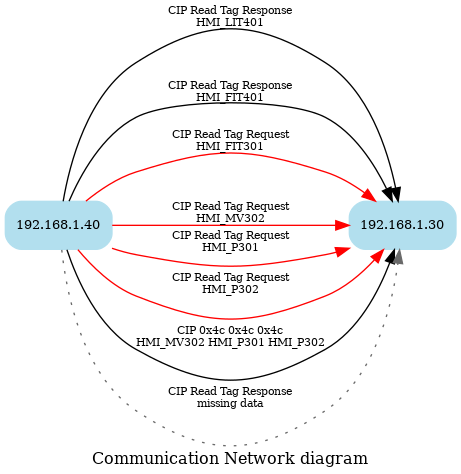
\includegraphics[scale=0.60]{chap4/4_network_graph_example.png}
	\caption{Network Communications between 192.168.1.40 (Source) and 192.168.1.30 (Destination)}
	\label{fig:4_network_graph_example}
\end{figure}

The graph illustrates the network communications between the source IP address 192.168.1.40 and the destination IP address 192.168.1.30. Each arrow represents a communication between these IP addresses, showcasing the flow and direction of the interactions. The red arrows indicate requests initiated by the source IP address towards the destination IP, while the black arrows represent responses sent by the source IP in response to previous requests made by the destination IP. The gray dotted arrows represent responses for which the corresponding request is missing or unavailable for some reason. Overall, the graph distinguishes the different types of communications and provides insights into the request-response dynamics between the source and destination IP addresses. The graph is automatically generated and saved within the\\ 
\texttt{\$(project\_dir)/network-analysis/data} directory.

\bigskip
In terms of the textual output, we can observe how the same data is represented. The communications exchanged between the two PLCs are displayed more prominently, allowing for a clearer understanding. Unlike the graph, the textual representation includes a column on the right-hand side, indicating the number of communications for each type of request. This provides a more distinct perspective on the network behavior within an industrial control system that utilizes, in this case, the CIP protocol for its communications.

\begin{figure}[ht]
	\centering
	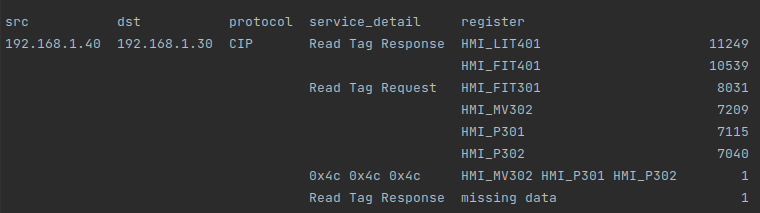
\includegraphics[scale=0.50]{chap4/network_text_output.png}
	\caption{Network Communications between 192.168.1.40 (Source) and 192.168.1.30 (Destination) in textual mode}
	\label{fig:4_network_textual_example}
\end{figure}

As previously mentioned, the textual data is stored in a CSV dataset located in the \texttt{\$(project\_dir)/network-analysis/data} directory.

\subsection{Phase 1: Data Pre-processing}
\label{subsec:improve_preprocessing}
\textit{Data Pre-processing phase} is probably the most delicate and significant one: depending on how large the industrial system to be analyzed is, the data collected, and how it is enriched using the additional attributes, the subsequent system analysis will provide more or less accurate outcomes.

\bigskip
The previous tool has several limitations, particularly at this stage. It does not allow for the isolation of a subsystem, either in terms of time or the number of PLCs to be analyzed. The system is considered as a whole without the ability to focus on specific subsystems. Additionally, many of the additional attributes had to be manually added, and for the ones entered automatically, there is no way to specify the register type to associate them with.\newline
The combination of these limitations, along with the presence of hardcoded references to attributes and registers in the tool's code, makes the analysis of the system more challenging. Furthermore, it compromises the accuracy and reliability of the obtained results in terms of both quantity and quality.

\bigskip
In the proposed framework, these issues have been addressed by incorporating new features. Firstly, the framework allows for the selection of a subsystem from the command line based on both temporal criteria and the specific PLCs to be included. This enables more focused and targeted analysis. Additionally, we have revamped the process of enriching the resulting dataset by eliminating manual entry of additional attributes. Instead, users now have the flexibility to determine the type of additional attribute to associate with a specific register.\newline
Furthermore, after the pre-processing stage, a preliminary analysis can be conducted on the resulting dataset. This analysis aims to identify the registers that are associated with actuators, measurements, and hardcoded setpoints or constants. It provides insights into the dataset and helps in refining the enrichment step. The parameters for this analysis can be configured in the \textit{config.ini} file, allowing for customization and fine-tuning of the process.\newline \newline 
In the upcoming sections, we will delve into a more comprehensive examination of the achievements made in this framework.

\subsubsection{Subsystem Selection}
\label{subsubsec:4_select_subsystem}

In the previous tool, the datasets for each individual PLC in CSV format were required to be placed in a specific directory that was hardcoded in the script. The script would then merge and enrich these datasets to generate a single output dataset representing the complete process trace of the industrial system. However, the script did not provide options to select specific PLCs for analysis or define a temporal range for analysis. This lack of flexibility made the analysis more complex, especially when dealing with \textit{transient states} (i.e., general statea in which the industrial system is still initializing before actually reaching full operation) or when focusing on specific parts of the industrial system during certain periods of interest. The fixed dataset structure also may increase the number of variables that could be analyzed.\newline
Furthermore, the previous tool did not allow for specifying an output CSV file to save the resulting dataset. Each dataset creation and enrichment operation would overwrite the previous file, making it inconvenient for comparisons between different execution traces unless the files were manually renamed.

\bigskip
The proposed framework addressed these issues by introducing improvements. First of all, in the general \textit{config.ini} file there are some general default settings about paths, and among them the one concerning the directory where to place the datasets of the individual PLCs to be processed. In addition to this option, there are other ones that define further aspects related to the operations performed in this phase. Listing \ref{lst:config_ini_preproc} shows the settings in question: 

\begin{lstlisting}[language=bash, numbers=none, caption=Paths and parameters for the Pre-processing phase in \textit{config.ini} file, label=lst:config_ini_preproc]	
	[PATHS]
	root_dir = /home/marcuzzo/UniVr/Tesi
	project_dir = %(root_dir)s/PLC-RE
	net_csv_path = %(root_dir)s/datasets_SWaT/2015/Network_CSV
	
	[PREPROC]
	raw_dataset_directory = datasets_SWaT/2015 # Directory containg datasets
	dataset_file = PLC_SWaT_Dataset.csv # Default output dataset
	granularity = 10  # slope granularity
	number_of_rows = 20000  # Seconds to consider
	skip_rows = 100000  # Skip seconds from beginning
\end{lstlisting}
At the same time, the user has the option to specify these settings via the command line using the new Python script called \texttt{mergeDatasets.py}, located in the \texttt{pre-processing} directory of the project. Any options provided through the command line will override the default settings specified in the \textit{config.ini} file. These options are:

\begin{itemize}
	\item \textbf{-s} or \textbf{{-}{-}skiprows:} initial transient period (expressed in seconds) to be skipped. This option is useful in case the system has an initial transient or the analyzer wishes to start the analysis from a specific point in the dataset;
	
	\item \textbf{-n} or \textbf{{-}{-}nrows:} time interval under analysis, expressed in terms of the number of rows in the dataset.\newline
	This option makes a \textbf{selection} on the data of the dataset;
	
	\item \textbf{-p} or \textbf{{-}{-}plcs:} PLCs to be merged and enriched. The user can specify the desired PLCs by indicating the CSV file names of the associated datasets with no limitations on number.\newline
	This option makes a \textbf{projection} on the data of the dataset.
	
	\item \textbf{-d} or \textbf{{-}{-}directory:} performs the merge and enrichment of all CSV files contained in the directory specified by user, overriding the default setting in \textit{config.ini}. It is in fact the old functionality of the previous tool, maintained here to give the user more flexibility and convenience in case he wants to perform the analysis on the whole system. This is also the default behavior in case the \texttt{-p} option is not specified.
	
	\item \textbf{-o} or \textbf{{-}{-}output:} specifies the name of the file in which the obtained dataset will be saved. It must necessarily be a file in CSV format.
	
	\item \textbf{-g} or \textbf{{-}{-}granularity:} specifies a granularity (expressed in seconds) that will be used to calculate the measurement slope during the dataset enrichment phase. We will discuss this later in Section \ref{subsubsec:4_dataset_enrichment}.
\end{itemize}

\subsubsection{Dataset Enrichment}
\label{subsubsec:4_dataset_enrichment}
After a step in which a function is applied to each PLC-related dataset to eliminate its unused registers within the system \footnote{This is especially true if the Modbus register scan has been performed, in which ranges of registers are scanned: it is assumed that unused registers have constant value zero}, the \textbf{dataset enrichment operation} is performed.\newline
This operation differs from the previous version not only in the fact that it is performed on each individual dataset and not on the resulting dataset, but also in the additional attributes: not only are they greater in number, but they are automatically calculated and inserted by the \texttt{mergeDatasets.py} script into the dataset and, most importantly, it is possible to decide through the parameters in the \textit{config.ini} configuration file under the \texttt{[DATASET]} section to which registers these attributes should be assigned. \newline
In Listing \ref{lst:4_enrich_params} we can see the list of additional attributes and how they should be associated with the registers of the dataset:

\begin{lstlisting}[language=Python,numbers=none,caption={\texttt{config.ini} parameters for dataset enriching},label=lst:4_enrich_params]
	[DATASET]
	timestamp_col = Timestamp
	max_prefix = max_
	min_prefix = min_
	max_min_cols_list = lit|ait|dpit
	prev_cols_prefix = prev_
	prev_cols_list = mv[0-9]{3}|p[0-9]{3}
	trend_cols_prefix = trend_
	trend_cols_list = lit
	trend_period = 150
	slope_cols_prefix = slope_
	slope_cols_list = lit
\end{lstlisting}
Following is a brief explanation of the parameters just seen:

\begin{description}
	\item[\texttt{timestap\_col}] indicates the name of the column that contains the data timestamps. This parameter is used not only in this phase, but is also referred to in the Process Mining phase. In the previous work, this parameter was hardcoded and not configurable (and thus causing errors if the system being analyzed changed)
	
	\item[\texttt{max\_prefix}, \texttt{min\_prefix}, \texttt{max\_min\_cols\_list}] refer to any relative maximum or minimum values (\textit{relative setpoints}) of one or more measures and that can be found and inserted as new columns within the dataset. The first two parameters indicate the prefix to be used in the column names affected by this additional attribute, while the third specifies of which type of registers we want to know the maximum and/or minimum value reached (several options can be specified using the logical operator \texttt{|} - or).\newline 
	If, for example, we want to know the maximum value of the registers associated with the tanks, indicated in the iTrust SWaT system by the prefix \texttt{LIT}, we only need to specify the necessary parameter in the \textit{config.ini} file, so \texttt{max\_min\_cols\_list = lit}.\newline
	The result will be to have in the dataset thus enriched a new column named \texttt{max\_P1\_LIT101}.
	
	\item[\texttt{prev\_cols\_prefix}, \texttt{prev\_cols\_list}]  refer to the values at the previous time instant of the registers specified in \texttt{prev\_cols\_list}. It is possible to specify registers using \textit{regex}, as in the example shown. It may be useful in some cases to have this value available to check, for example, when a change of state of a single given actuator occurs.  The behavior of these parameters is the same as described in the point above.
	
	\item[\texttt{slope\_cols\_prefix}, \texttt{slope\_cols\_list}] are related to the calculation of the slope of a specific register that contains numeric values (usually a measure), that is, its trend. Slope calculation makes little sense on booleans. The slope can be \textbf{ascending} (if its value is greater than zero), \textbf{descending} (if less than zero) or \textbf{stable} (if approximately equal to zero). We will delve into the details of slope calculation in the following paragraph, as it pertains to the attributes \texttt{trend\_cols\_prefix}, \texttt{trend\_cols\_list}, and \texttt{trend\_period}.
\end{description}

Initially, the parameters for registers to be associated with each additional attribute may be left blank, as we may not have prior knowledge about the system and are unsure about which registers correspond to actuators, measurements, or other attributes. This information can be obtained from the preliminar analysis that follows the merging of datasets. The analysis, performed based on user's choice, provides indications on potential sensors, actuators, and other relevant information. These indications help the user set the desired values in the \textit{config.ini} file and refine the enrichment process by re-launching the \texttt{mergeDatasets.py} script.

\paragraph{Slope Calculation}
\label{par:4_slope_calculation}
The \textit{slope} is an attribute that represents the \textbf{trend} of the measurement being considered. It is particularly useful, in our context, during the inference and invariant analysis phase to gather information about the trend under specific conditions. The slope can generally be classified as \textbf{increasing} (slope > 0), \textbf{decreasing} (slope < 0), or \textbf{stable} (slope = 0).\newline
Normally, the slope is calculated through a simple mathematical formula: given an interval \textit{a}, \textit{b} relative to the measurement \textit{l}, the slope is given by the difference of these two values divided by the amount of time \textit{t} that the measurement takes to reach \textit{b} from \textit{a}:

\[slope = \frac{l(b) -l(a)}{t(b) - t(a)}\]

In the proposed framework, similar to the previous tool, this time interval (the granularity) can be adjusted to be either long or short. The choice of granularity depends on the desired accuracy of the slope calculation. A lower granularity will provide a slope that closely reflects the actual measurement trend, while a higher granularity will result in flatter slope data. Each time interval within which the measurement is divided corresponds to a slope value. These slopes are calculated and added as additional attributes in the dataset. Later on, these slope values are used to determine the trend of the measurement in specific situations or conditions.

\bigskip
Calculating the slope directly from the raw measurement data can be a suitable approach for systems where the measurements are not heavily influenced by \textbf{perturbations}. Perturbations, such as liquid oscillations in a tank during filling and emptying phases, can lead to fluctuating readings of the level. In such cases, maintaining a low granularity can provide a more accurate calculation of the overall trend that closely aligns with the actual measurement trend. The tanks of Ceccato et al.'s testbed are an example where this holds true.\newline
However, if perturbations significantly affect the measurement readings, calculating the slope on individual time intervals may result in an inaccurate trend definition, irrespective of the chosen granularity. In such cases, the fluctuating nature of the measurements due to perturbations can introduce errors in the slope calculation, making it less reliable as an indicator of the actual trend.

\bigskip
Figure \ref{fig:4_slope_comparison} demonstrates this assertion: the measurement, in blue, refers to the \texttt{P1\_LIT101} tank of the iTrust SWaT system; in red, the slope calculation related to the measurement with three different granularities: 30 (Figure \ref{subfig:4_slope_g30_nodecomp}), 60 (Figure \ref{subfig:4_slope_g60_nodecomp}) and 120 seconds (Figure \ref{subfig:4_slope_g120_nodecomp}). It is noticeable that as the granularity increases, the slope values flatten. Moreover, in the time interval between seconds 1800 and 4200, the level of \texttt{P1\_LIT101} exhibits a predominantly increasing trend, yet the calculated slope values fluctuate between positive and negative. Consequently, during the invariant analysis, the overall increasing trend may not be detected, resulting in a loss of information.\newline

\begin{figure}[H]
	\centering
	\begin{subfigure}{0.90\textwidth}
		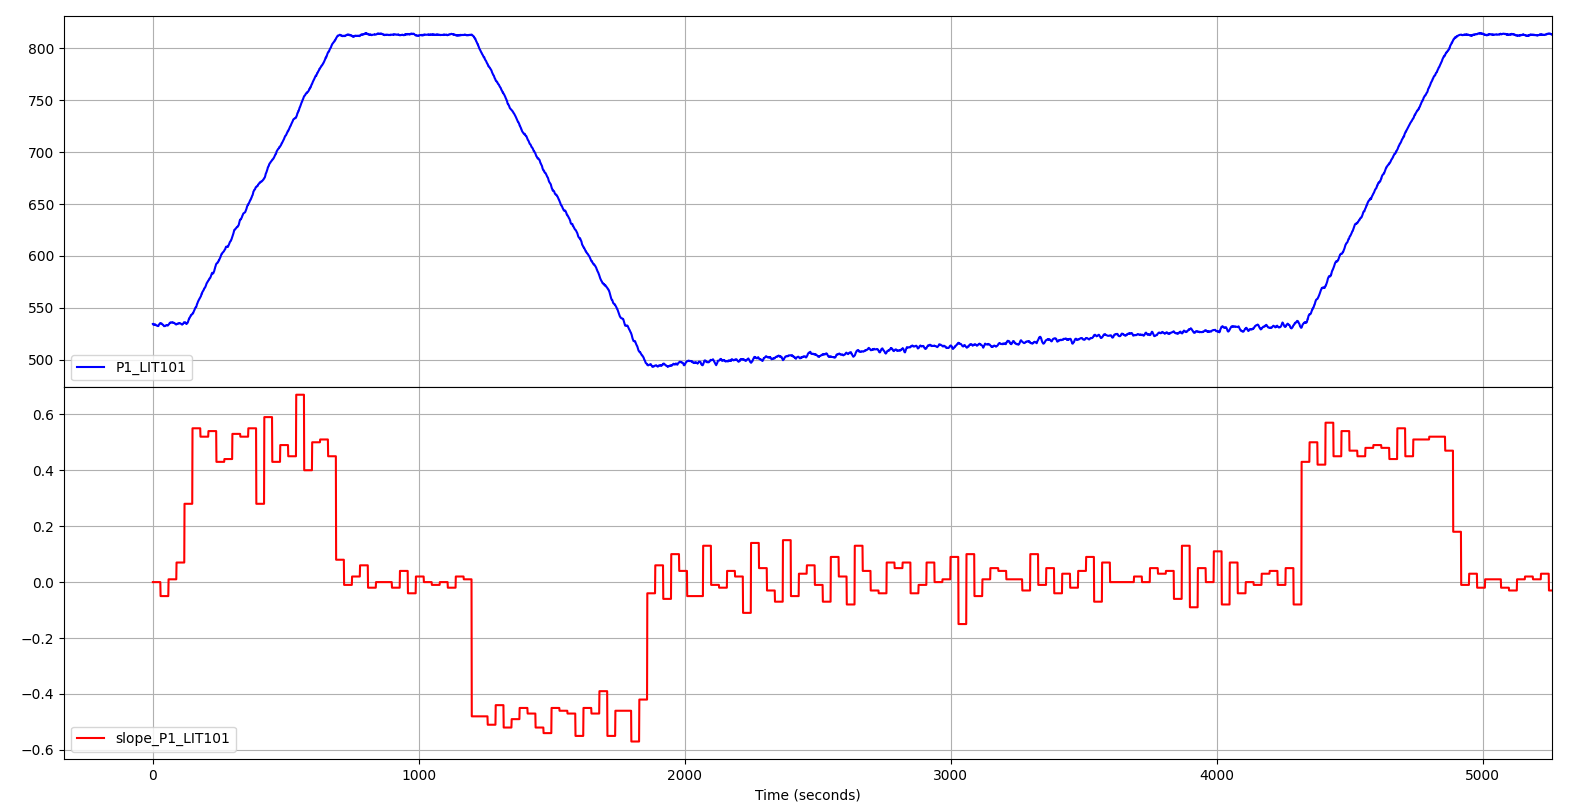
\includegraphics[width=\textwidth]{chap4/slope_nodecomp_g30_2.png}
		\caption{}
		\label{subfig:4_slope_g30_nodecomp}
	\end{subfigure}
	\hfill
	\begin{subfigure}{0.90\textwidth}
		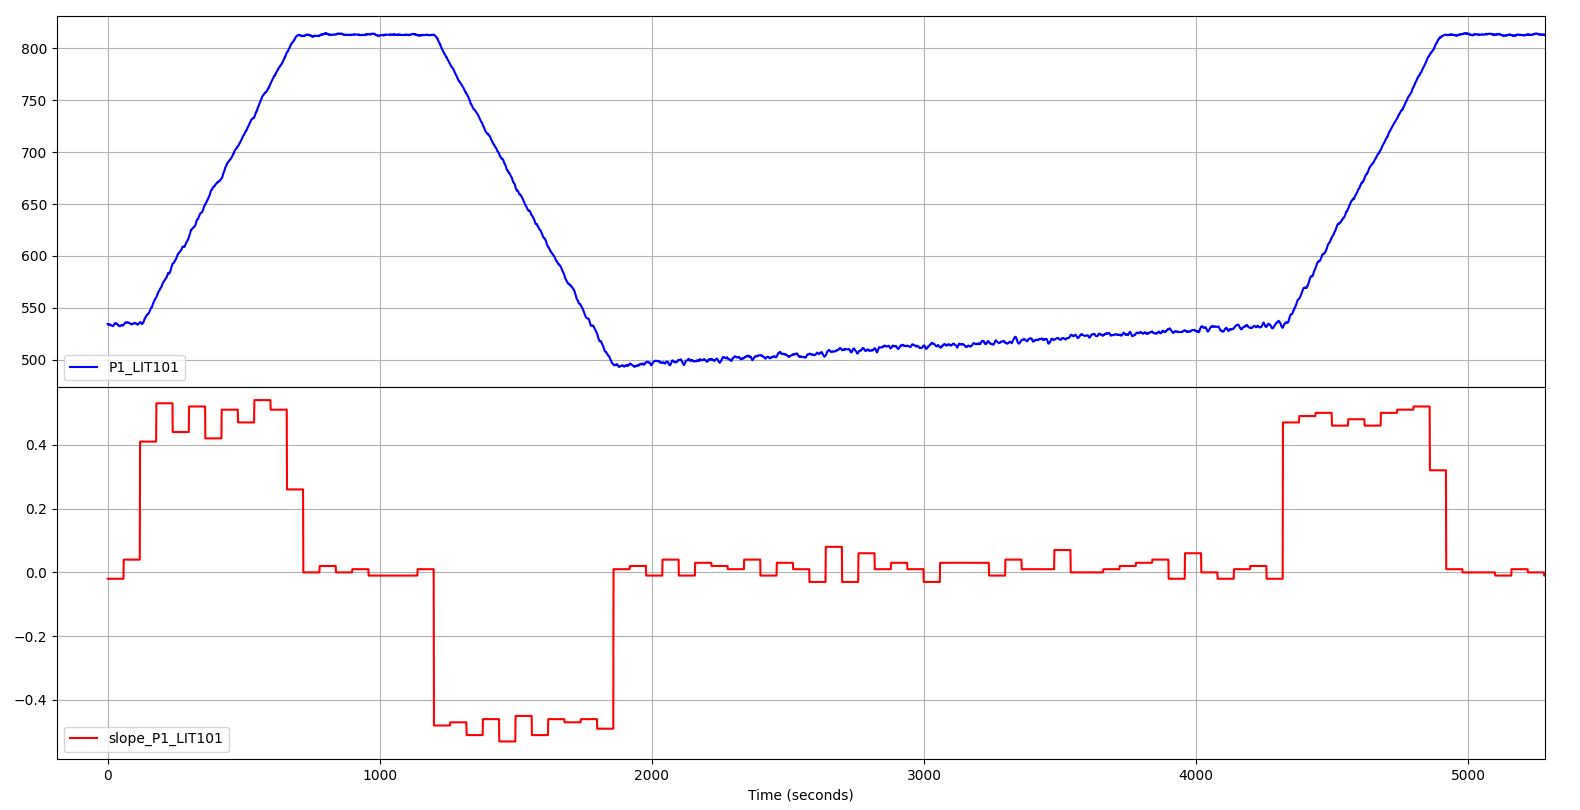
\includegraphics[width=\textwidth]{chap4/slope_nodecomp_g60_2.png}
		\caption{}
		\label{subfig:4_slope_g60_nodecomp}
	\end{subfigure}
	\begin{subfigure}{0.90\textwidth}
		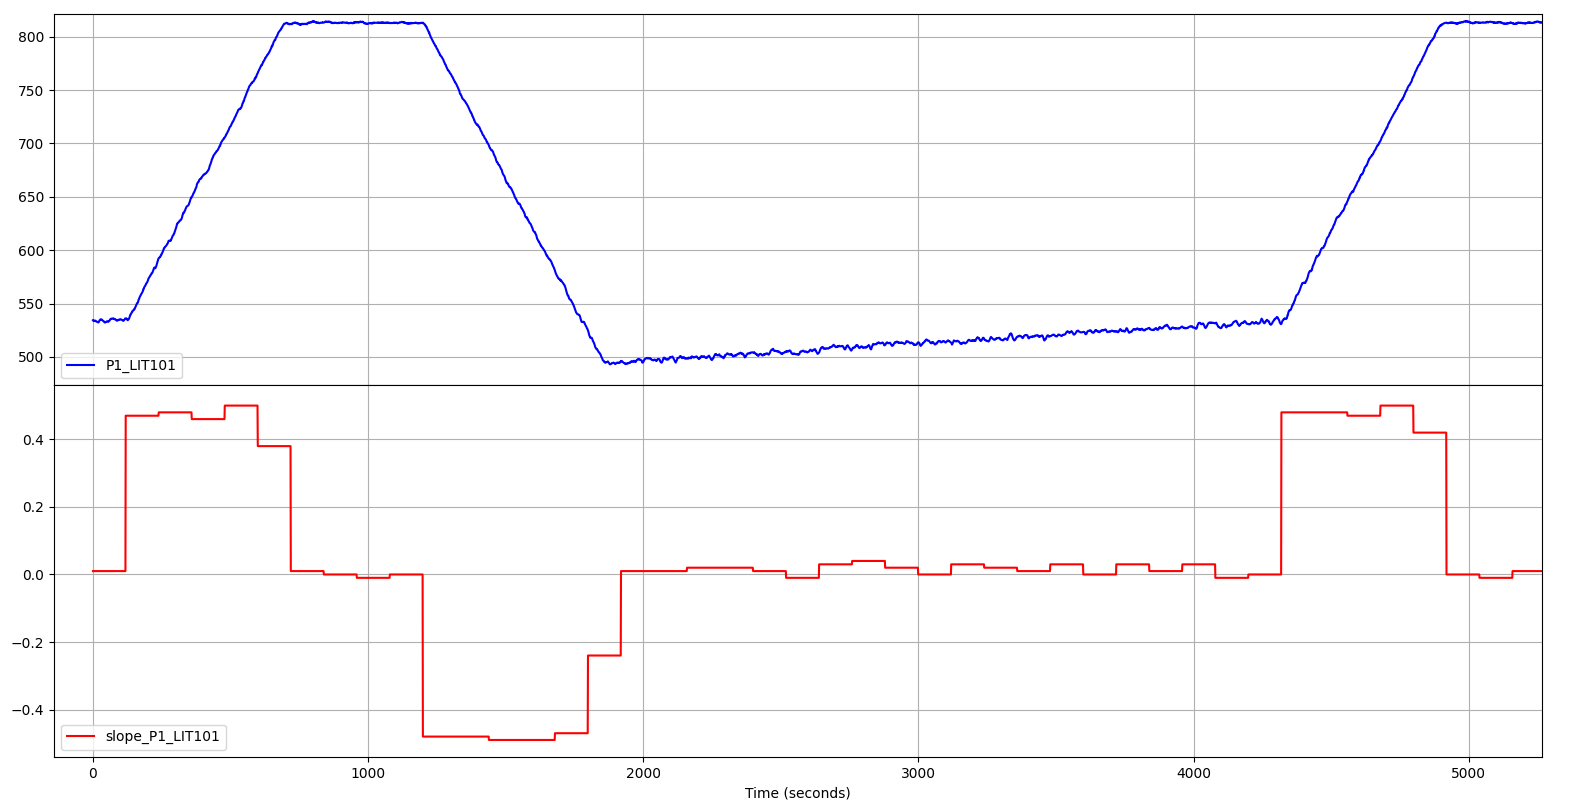
\includegraphics[width=\textwidth]{chap4/slope_nodecomp_g120_2.png}
		\caption{}
		\label{subfig:4_slope_g120_nodecomp}
	\end{subfigure}
	\caption{Slope comparison with granularity 30 (a), 60 (b) and 120 seconds (c)}
	\label{fig:4_slope_comparison}
\end{figure}

\noindent The previous tool did not take into account the possibility of having strongly perturbed data, which presented a challenge that we needed to address in the development of the proposed framework.

\bigskip
The solution to this problem involves applying techniques to reduce the "noise" in the data, aiming to achieve a more linear trend in the measurement curve. By minimizing the effects of perturbations, we can calculate slopes more accurately.\newline
There are various methods available for smoothing out noise in the data. In our framework, we focused on two commonly used approaches found in the literature: \textbf{polynomial regression} and \textbf{seasonal decomposition}. In addition to these two methods, we also explored the use of a \textbf{line simplification algorithm}.\newline \newline
\textit{Polynomial regression} \cite{polynomial_regression} is a technique that allows us to create a filter to reduce the impact of noise on the data. By fitting a polynomial function to the measurements, we can obtain a smoother curve that captures the underlying trend while minimizing the effects of perturbations.\newline
\textit{Seasonal decomposition} \cite{seasonal_decomposition}, specifically the part related to trending, is another method we explored. It involves decomposing the time series into different components, such as trend, seasonality, and residual. By isolating the trend component, we can obtain a cleaner representation of the underlying pattern in the data.\newline
\textit{Line simplification algorithms} \cite{line_simplification_algo} aim to reduce the complexity of a polyline or curve by approximating it with a simplified version composed of fewer points. By selectively removing redundant or less significant points, line simplification algorithms help reduce storage space and computational requirements while preserving the overall shape and characteristics of the original line.\newline
Regarding polynomial regression, we evaluated the use of the \textbf{Savitzky-Golay filter} \cite{savgol} as a smoothing technique. For seasonal decomposition, we explored the \textbf{Seasonal-Trend decomposition using LOESS} (STL) method \cite{stl_decomp}. For the line simplification algorithm, we specifically considered the \textbf{Ramer-Douglas-Peucker} (RDP) algorithm \cite{ramer-douglas-peucker}.\newline \newline
%For lacking of space we are unable to provide a detailed description of the polynomial regression and seasonal decomposition techniques in this context. We recommend referring to the bibliographical notes or relevant literature for a more comprehensive understanding of these methods. 
Figure \ref{fig:4_smoothing_comparison} shows a quick graphical comparison of these techniques compared with the original data. The solution adopted is the \textit{STL decomposition} method, which effectively reduces noise compared to the Savitzky-Golay filter. However, it should be noted that this method may introduce some delay in certain parts of the data, as is typically observed in similar algorithms. Despite its apparent effectiveness, the RDP algorithm fails to accurately approximate sections where the measurement level remains relatively stable. Consequently, it yields incorrect slope estimations, causing a loss of valuable information about the system.

\begin{figure}[H]
	\centering
	\begin{subfigure}{0.48\textwidth}
		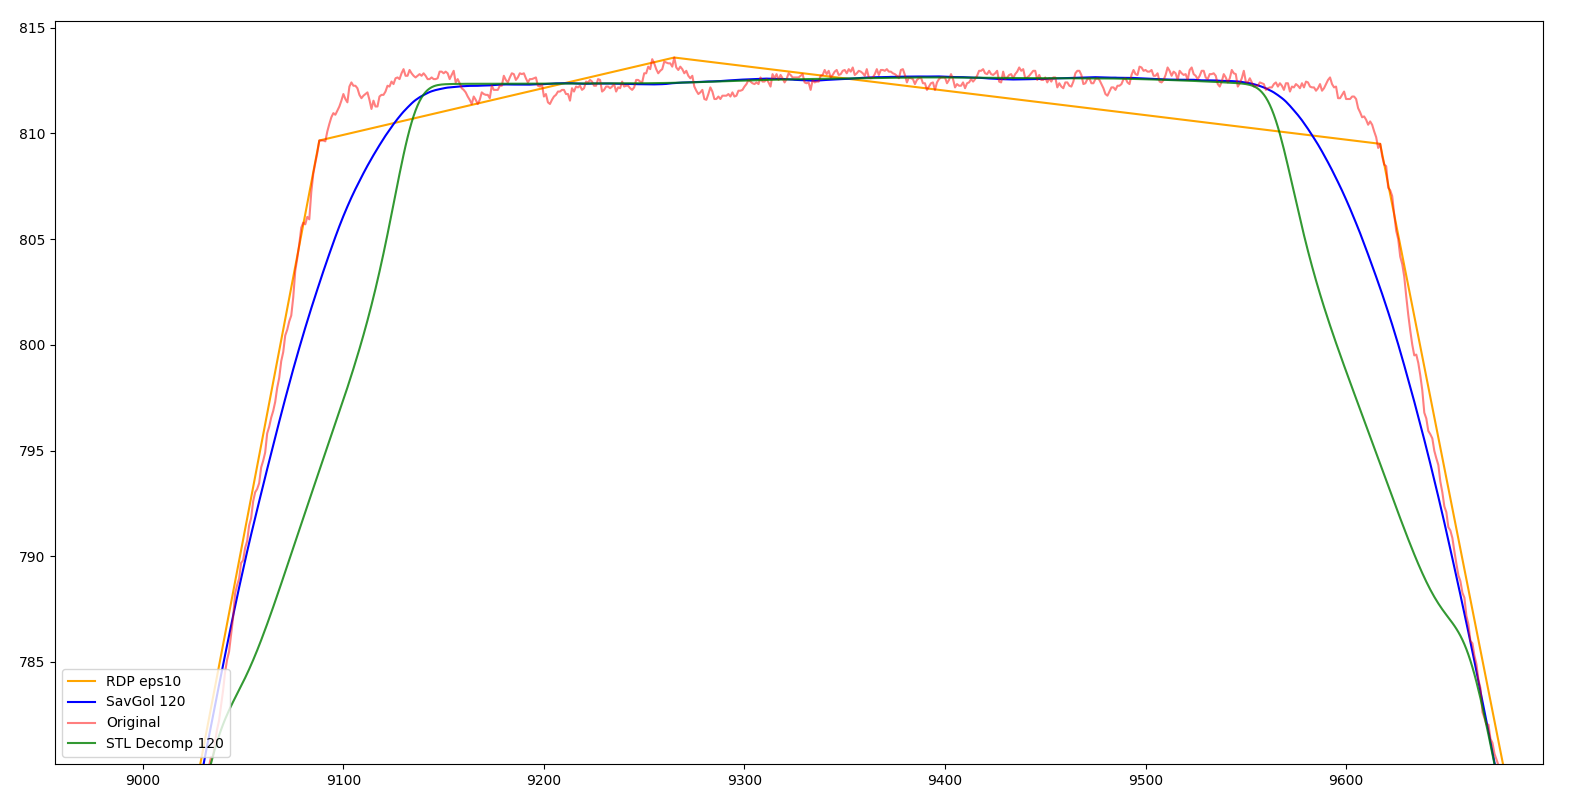
\includegraphics[width=\textwidth]{chap4/confronto_RDP_SavGol_STL_1.png}
		\caption{}
		\label{subfig:4_smoothing1}
	\end{subfigure}
	\hfill
	\begin{subfigure}{0.48\textwidth}
		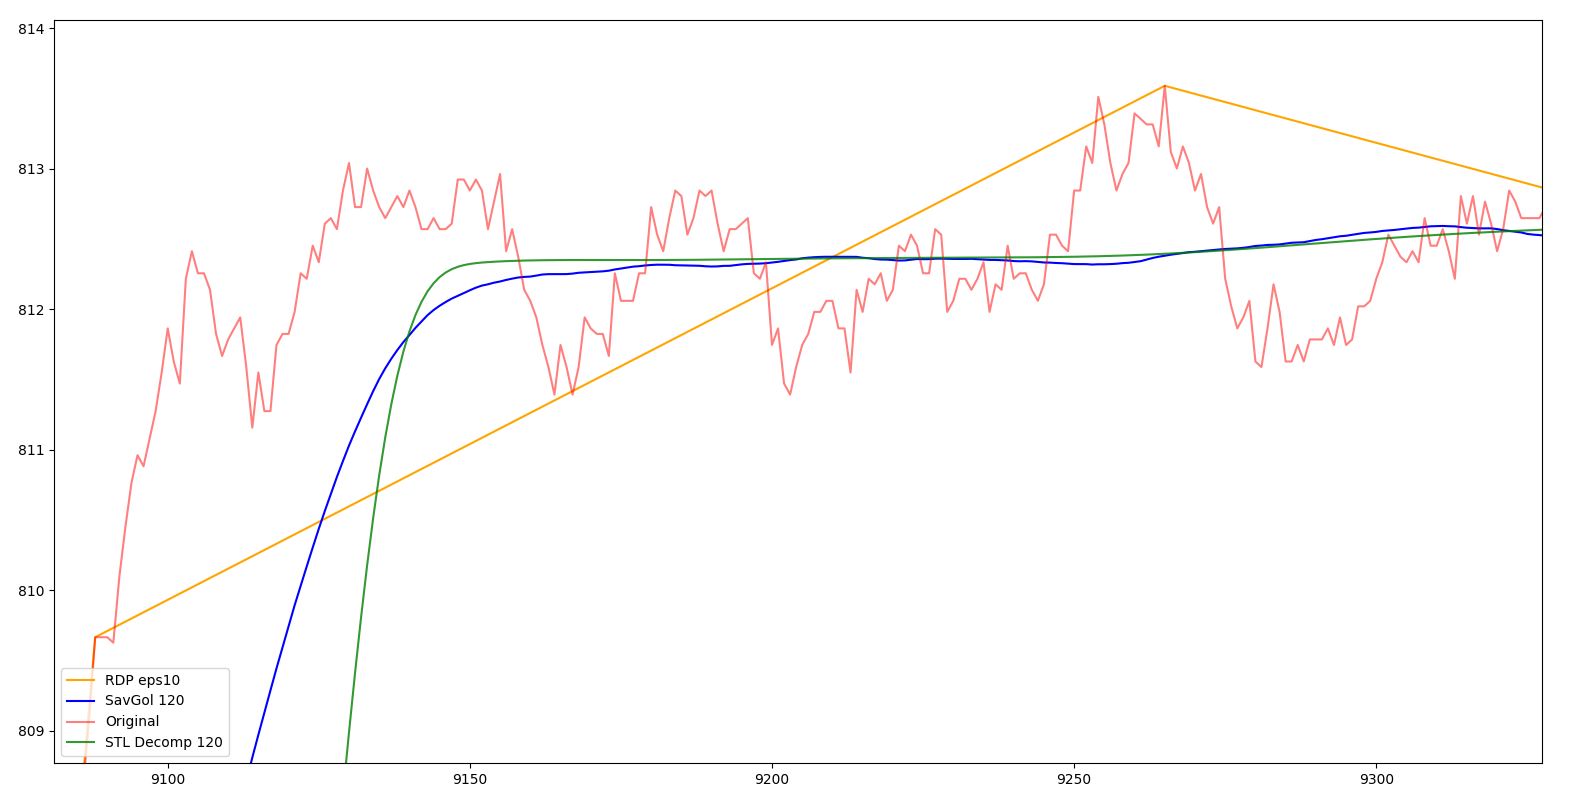
\includegraphics[width=\textwidth]{chap4/confronto_RDP_SavGol_STL_2.png}
		\caption{}
		\label{subfig:4_smoothing2}
	\end{subfigure}
	\begin{subfigure}{0.48\textwidth}
		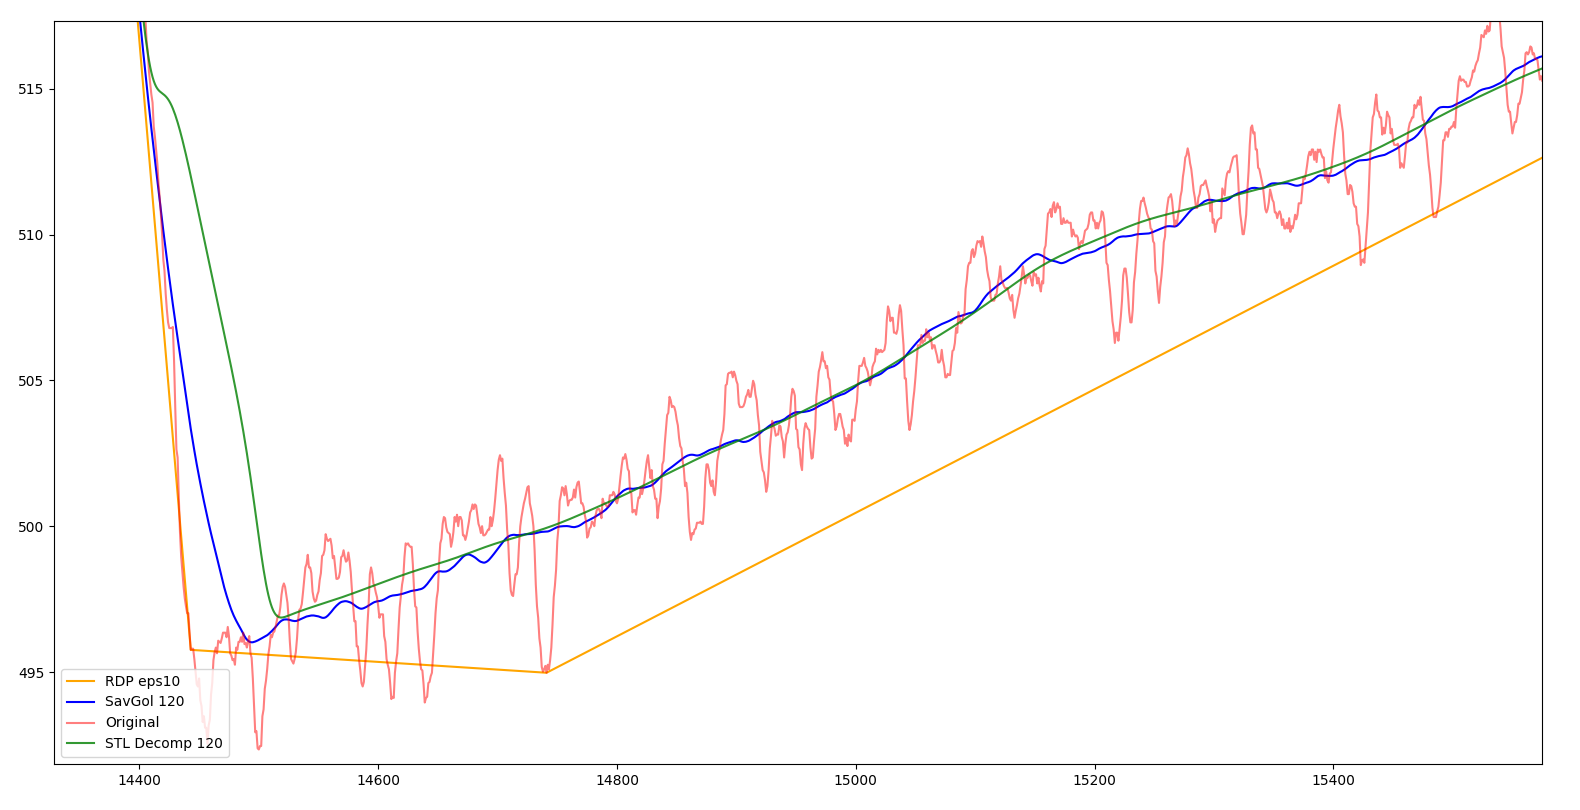
\includegraphics[width=\textwidth]{chap4/confronto_RDP_SavGol_STL_3.png}
		\caption{}
		\label{subfig:4_smoothing3}
	\end{subfigure}
	\hfill
	\begin{subfigure}{0.48\textwidth}
		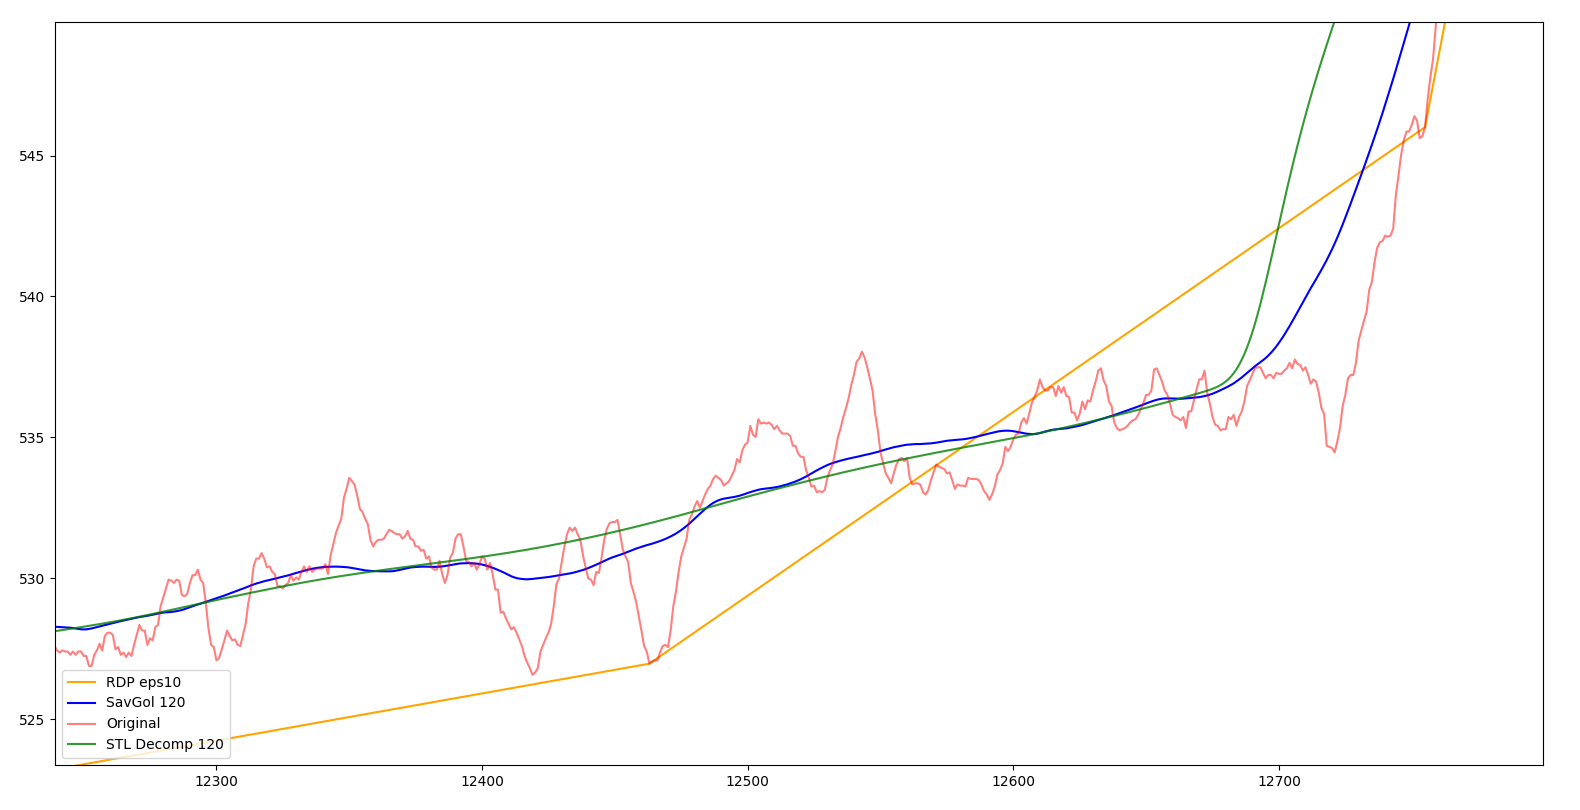
\includegraphics[width=\textwidth]{chap4/confronto_RDP_SavGol_STL_4.png}
		\caption{}
		\label{subfig:4_smoothing4}
	\end{subfigure}
	\caption{Savitzky-Golay filter (blue line), STL decomposition (green) and RDP algorithm (orange) comparison}
	\label{fig:4_smoothing_comparison}
\end{figure}
By applying the STL decomposition, we observe a notable enhancement in slope calculation even when using a low granularity. Figure \ref{fig:4_STL_decomp_results} demonstrates that, with the same granularity as shown in Figure \ref{subfig:4_slope_g30_nodecomp}, the slope values, albeit exhibiting fluctuations, consistently align with the underlying trend of the data curve. The introduced lag resulting from the decomposition's periodicity is responsible for the observed delay.

\begin{figure}[ht]
	\centering
	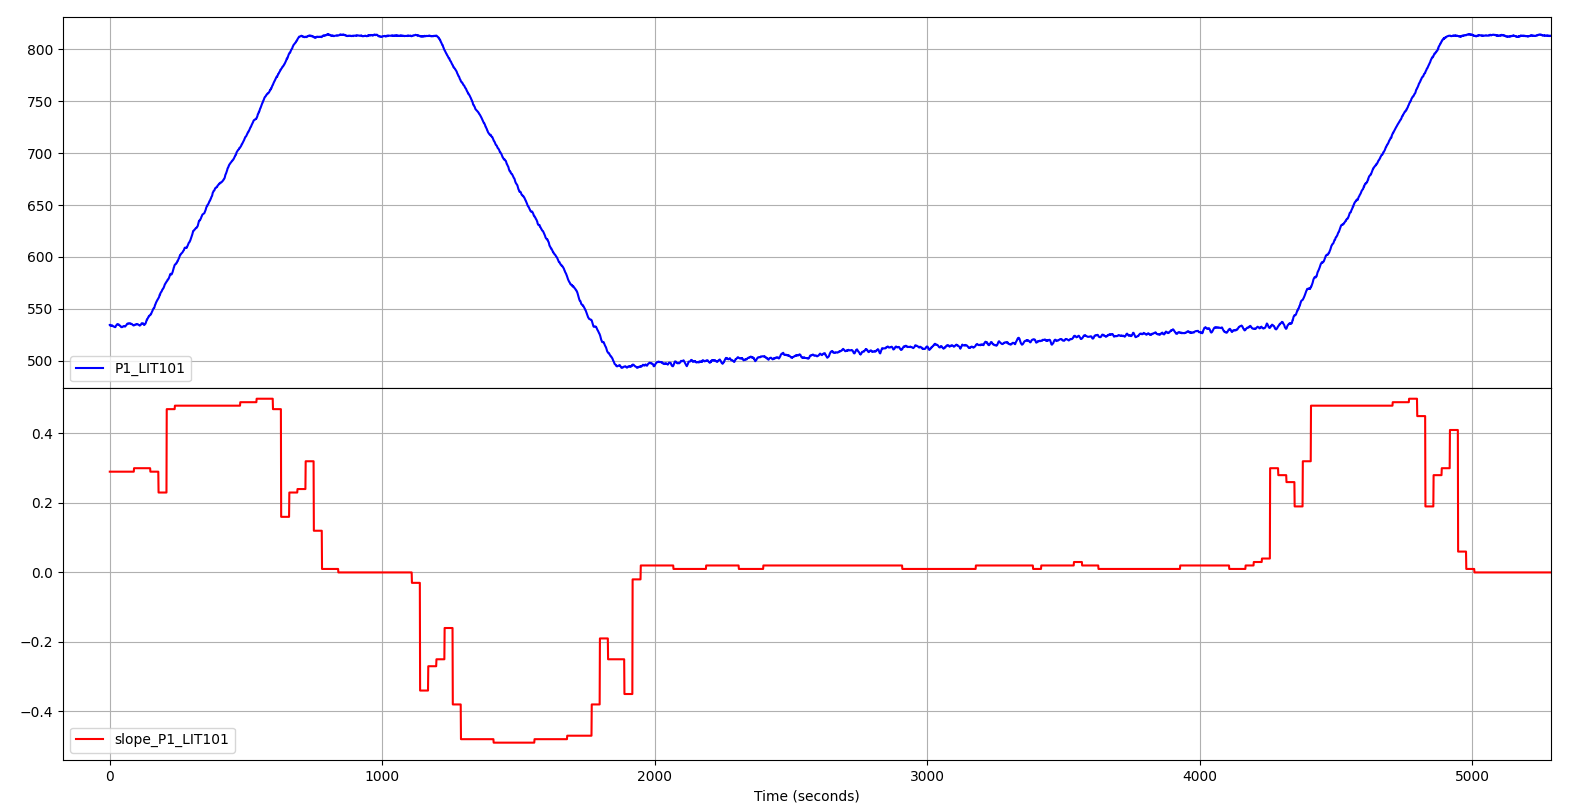
\includegraphics[scale=0.35]{chap4/slope_STL_g30_2.png}
	\caption{Slope after the application of the STL decomposition}
	\label{fig:4_STL_decomp_results}
\end{figure}
The periodicity, which defines the sampling time window for decomposition and the level of noise smoothing, can be configured using the \texttt{trend\_period} directive in the \textit{config.ini} file.\newline
During the slope calculation, the analysis will be performed on the data from the additional measurement trend attributes specified in the \texttt{trend\_cols\_list} directive of the configuration file, rather than on the original unfiltered data.

\bigskip
To ensure proper interpretation by Daikon, the decimal values representing the calculated slopes are converted into \textbf{three numerical values}: -1, 0, and 1. These values correspond to \textit{decreasing} (if the slope is less than zero), \textit{stable} (if it is equal to zero), and \textit{increasing} (if it is greater than zero) trends, respectively. Figure \ref{fig:4_slope_daikon} displays the modified slopes along with the curve obtained from the STL decomposition:

\begin{figure}[ht]
	\centering
	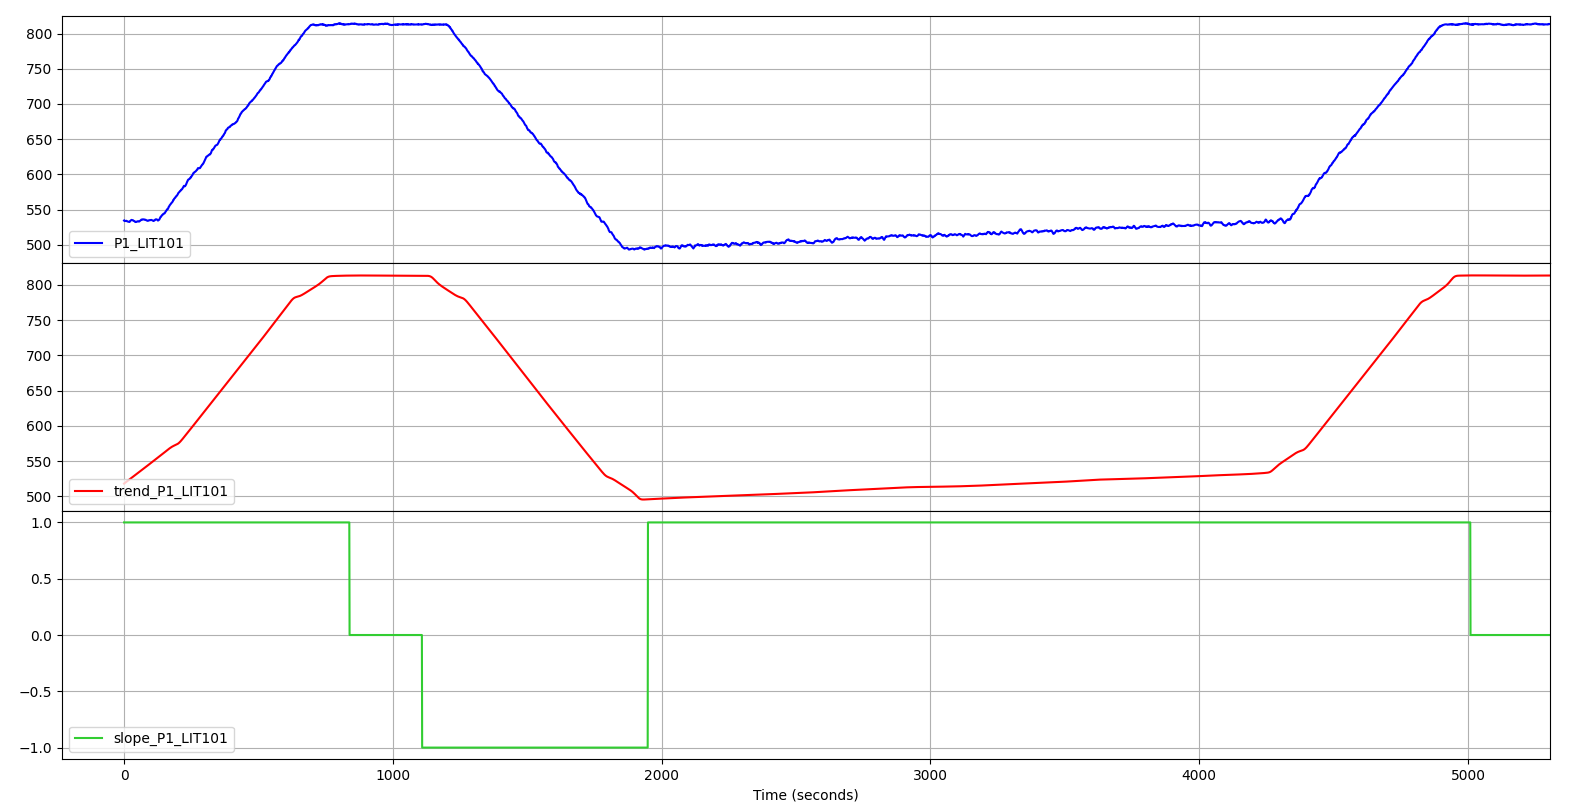
\includegraphics[scale=0.35]{chap4/slope_STL_bin_g30_2b.png}
	\caption{The new slope representation (green line) and the smoothed measurement data obtaind with the STL decomposition (red)}
	\label{fig:4_slope_daikon}
\end{figure}

\subsubsection{Datasets Merging}
\label{subsubsec:4_dataset_merging}
During this step, the datasets of the individual PLCs are merged, resulting in two separate datasets. The first dataset is enriched with additional attributes but excludes the timestamp column. This dataset is intended for inference and invariant analysis. The second dataset does not contain any additional data and is specifically used in the process mining phase.

\bigskip
By default, the enriched dataset will be saved in CSV format in the \texttt{\$(project-dir)/daikon/Daikon\_Invariants} directory. The other dataset, without additional data, will be saved in the \texttt{\$(project-dir)/process-mining/data directory}. It's worth noting that both paths can be configured in the \textit{config.ini} file. The dataset name can be specified in the \textit{config.ini} file or through the \texttt{-o} command-line option. When generating the dataset for process mining, the script will automatically add a \texttt{\_TS} suffix to the filename to indicate that it includes the timestamp. This flexibility allows the user to provide a different filename for each output, preventing overwriting of previous datasets. It enables the user to save the execution trace of the selected subsystem separately and utilize them in subsequent analysis phases.

\subsubsection{Preliminar Analysis of the Obtained Subsystem}
\label{subsubsec:4_brief_analysis}

After merging the datasets, the user has the option to perform an \textbf{optional analysis} of the resulting dataset to extract preliminary data. This analysis aims to gather basic information about the (sub)system and potentially refine the enrichment process. If the user chooses to proceed with the analysis, the \texttt{mergeDatasets.py} script invokes another Python script located in the \texttt{\$(project-dir)/pre-processing} directory called \texttt{system\_info.py}.\newline
Relying on an analysis based on a combination of Daikon and Pandas this script performs a quick analysis of the dataset allowing to \textbf{estimate}, albeit approximately, the \textbf{type of registers} (sensors, actuators, ...), also identifying possible maximum and minimum values of measurements and hardcoded setpoints. Furthermore, leveraging the use of the additional attribute \texttt{prev\_}, the \texttt{system\_info.py} script is capable of deriving measurement values corresponding to state changes of individual actuators. This allows for the identification of specific measurements associated with the activation or deactivation of certain actuators within the system.\newline
As the last information we have duration of actuator states for each cycle of the system: this information can be useful for making assumptions and conjectures about the behavior of an actuator in a specific state or, by observing the duration values of each cycle, highlighting anomalies in the system. \newline
Listing \ref{lst:4_brief_infos} shows an example of this brief analysis related to PLC1 of the iTrust SWaT system (for brevity, only one measurement is reported in the analysis of actuator state changes):

\begin{lstlisting}[language=bash,numbers=none,caption={Example of preliminar system analysis},label=lst:4_brief_infos]
	Do you want to perform a brief analysis of the dataset? [y/n]: y
	
	Actuators: 
	P1_MV101 [0.0, 1.0, 2.0]
	P1_P101 [1.0, 2.0]
	
	Sensors: 
	P1_FIT101 {'max_lvl': 2.7, 'min_lvl': 0.0}
	P1_LIT101 {'max_lvl': 815.1, 'min_lvl': 489.6}
	
	Hardcoded setpoints or spare actuators: 
	P1_P102 [1.0]
	
	Actuator state changes:
	       P1_LIT101  P1_MV101  prev_P1_MV101
	669     800.7170         0              2
	1850    499.0203         0              1
	4876    800.5992         0              2
	6052    498.9026         0              1
	9071    800.7170         0              2
	10260   499.1381         0              1
	13268   801.3058         0              2
	14435   498.4315         0              1
	17423   801.4628         0              2
	18603   498.1567         0              1
	
	P1_LIT101  P1_MV101  prev_P1_MV101
	677     805.0741         1              0
	4885    805.7414         1              0
	9079    805.7806         1              0
	13276   805.1133         1              0
	17432   804.4068         1              0
	
	P1_LIT101  P1_MV101  prev_P1_MV101
	1858    495.4483         2              0
	6060    497.9998         2              0
	10269   495.9586         2              0
	14443   495.8016         2              0
	18611   494.5847         2              0
	
	       P1_LIT101  P1_P101  prev_P1_P101
	118     536.0356        1             2
	4322    533.3272        1             2
	8537    542.1591        1             2
	12721   534.8581        1             2
	16883   540.5890        1             2
	
	P1_LIT101  P1_P101  prev_P1_P101
	1190    813.0031        2             1
	5395    813.0031        2             1
	9597    811.8256        2             1
	13776   812.7283        2             1
	17938   813.3171        2             1
	
	Actuator state durations:
	P1_MV101 == 0.0
	9  9  10  9  9  10  9  9  10  9
	
	P1_MV101 == 1.0
	1174  1168  1182  1160  1172
	
	P1_MV101 == 2.0
	669  3019  3012  3000  2981
	
	P1_P101 == 1.0
	1073  1074  1061  1056  1056
	
	P1_P101 == 2.0
	118  3133  3143  3125  3108
\end{lstlisting}

From these results we can draw the following conjectures: 

\begin{itemize}
	\item the \textbf{probable actuators} are \texttt{P1\_MV101} and \texttt{P1\_P101}. \texttt{P1\_MV101} has three states identified by the values 0, 1, and 2, suggesting it is a multi-state actuator. \texttt{P1\_P101} has two states identified by the values 1 and 2, indicating a binary actuator;
	
	\item there are \textbf{two probable measures}: \texttt{P1\_FIT101} and \texttt{P1\_LIT101}. \texttt{P1\_FIT101} has values ranging from 0 to 2.7, \texttt{P1\_LIT101} has values ranging from 489.6 to 815.1. Based on this information, a further conjecture can be made that \texttt{P1\_LIT101} represents a tank level measurement;
		
	\item apparently there is a probable \textbf{spare actuator}, \texttt{P1\_P102}, whose value is always 1. No related \textit{hardcoded setpoints} were found. From this information, another speculation can be made that the value 1 represents the \textbf{OFF state} for binary actuators, while the value 2 represents the \textbf{ON state};
	
	\item from the analysis of state changes we can derive some \textbf{relative setpoints}. For example, we observe that \texttt{P1\_P101} changes state from value 1 (OFF) to value 2 (ON) when the level of \texttt{P1\_LIT101} is approximately 813, and it changes from value 2 (ON) to 1 (OFF) when the level of \texttt{P1\_LIT101} is around 535. We can deduce that \texttt{P1\_P101} is responsible for emptying the tank;
	
	\item Regarding the actuators states duration, the very short duration of \texttt{P1\_MV101} in state 0 is observable: since we are unable, at this preliminary stage, to make assumptions about this, we will try to understand the behavior of the system in this actuator state in the next stages of the analysis.
\end{itemize}

The information obtained here can be used, as mentioned above, to refine the enrichment of the dataset by setting directives in the \texttt{[DATASET]} section of the \textit{config.ini} file, should this be empty or only partially set, or to make the first conjectures about the system, as we have just seen.

\bigskip
The \texttt{system\_info.py} file can also run in standalone mode if needed: it takes as command-line arguments the dataset to be analyzed, a list of actuators, and a list of sensors. For analysis related to state changes, the dataset must mandatorily be of the enriched type.

\subsection{Phase 2: Graphs and Statistical Analysis}
\label{subsec:4_improve_graphs}

The new \textit{graph analysis} arises from the need to give the user an overview of the (sub)system obtained in the previous pre-processing phase, identifying more easily the typology of the registers and grasping more effectively the relationships and the dynamics that may exist between the registers controlled by one or more PLCs, confirming the initial conjectures if the preliminar analysis described in the previous section has been performed, or making new ones thanks to the visual graph support. 

\bigskip
In Ceccato et al.'s framework, as mentioned in Section \ref{subsec:3_ceccato_limitations}, it was only possible to view the chart of one register at a time. While this allowed for the identification or hypothesis of the register type, it made it challenging to establish relationships with other components of the system and derive conjectures about their behavior. To address this limitation, there was a need for a new tool that could provide more information in a more accessible manner.

\bigskip
Initially, we considered adopting an approach similar to Figure \ref{fig:graph_analysis_prop3}, where all the graphs are displayed within a single plot. However, we soon realized that this solution was not feasible and could not be adopted. Figure \ref{fig:4_plot_comparison_1} helps to understand why.  

\begin{figure}[H]
	\centering
	\begin{subfigure}{0.48\textwidth}
		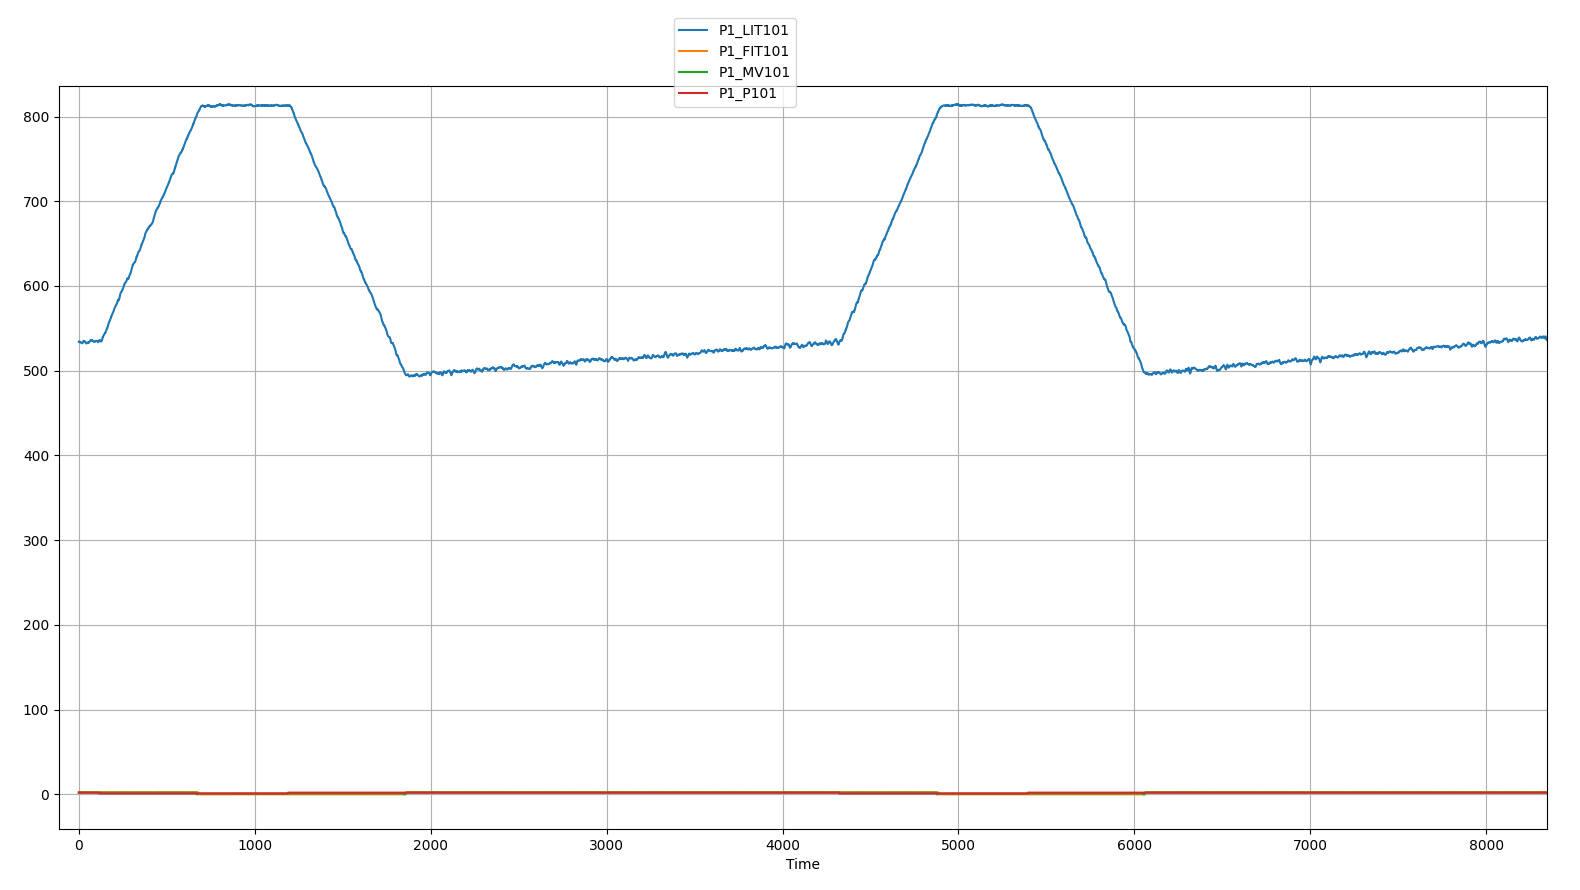
\includegraphics[width=\textwidth]{chap4/wrong_plot_1.png}
		\caption{}
		\label{subfig:4_wrong_plot}
	\end{subfigure}
	\hfill
	\begin{subfigure}{0.48\textwidth}
		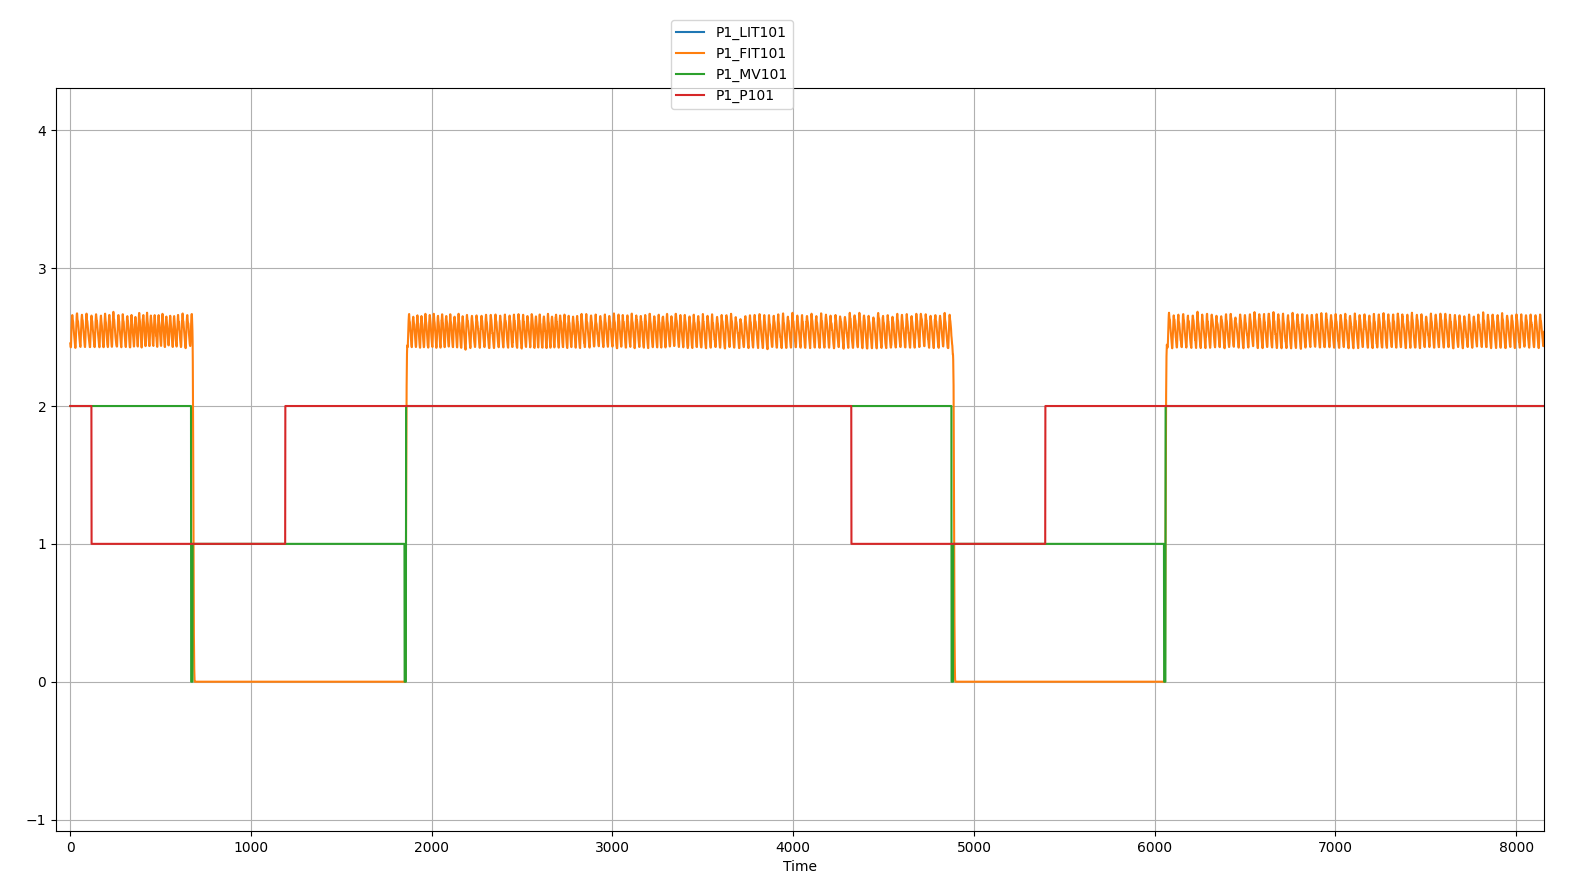
\includegraphics[width=\textwidth]{chap4/wrong_plot_2.png}
		\caption{}
		\label{subfig:4_wrong_plot_zoom}
	\end{subfigure}
	\caption{Plotting registers on the same y-axis}
	\label{fig:4_plot_comparison_1}
\end{figure}
Figure \ref{subfig:4_wrong_plot} highlights the main issue with this approach, which is the use of the same y-axis for all the charts, representing the values of individual registers. When the range between register values is wide, it can result in some charts appearing as a single flat line or becoming indistinguishable, making them difficult to read. Additionally, as shown in Figure \ref{subfig:4_wrong_plot_zoom}, when registers have similar values, the graphs can become confusing and harder to interpret.

\bigskip
The solution to this issue is simple and effective: the use of \textbf{subplots}. Basically, each register corresponds to a subplot of the graph that shares the time axis (the x-axis) with the other subplots, but keeps the y-axis of the values of each register independent. This maintains the readability and comprehensibility of the charts, while simultaneously being able to immediately grasp the relationships between them. In addition, by sharing the time axis, it is possible to zoom in on a particular area of one of the charts and automatically the other ones will be zoomed in as well, thus not losing any information and no connection between registers. Figure \ref{fig:4_graph_analysis} illustrates more clearly what has just been explained: the charts refer to the PLC1 registers of the iTrust SWaT system.

\begin{figure}[H]
	\centering
	\begin{subfigure}{0.9\textwidth}
		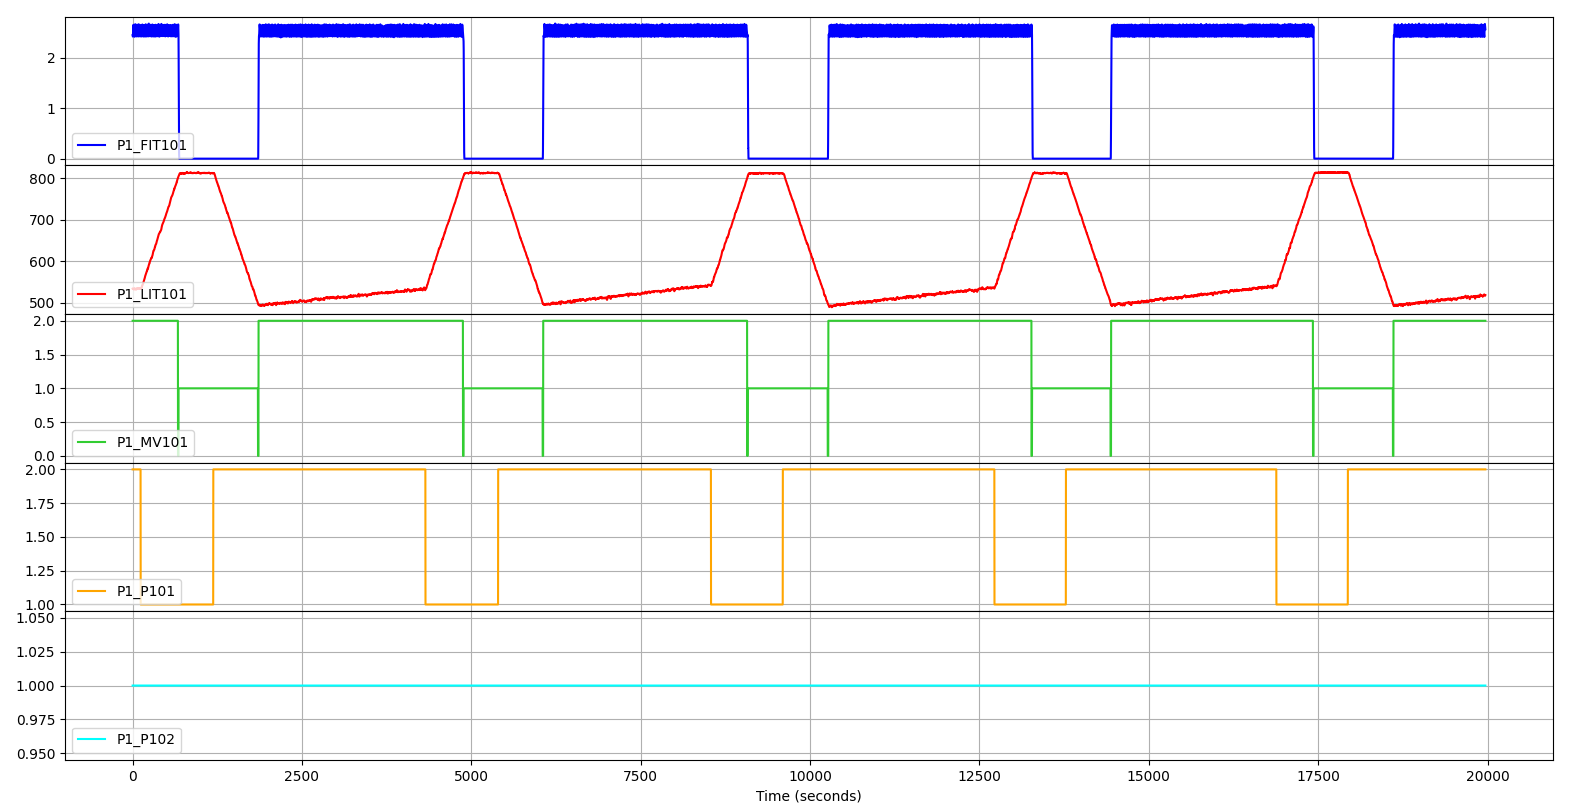
\includegraphics[width=\textwidth]{chap4/graph_analysis_plot_1.png}
		\caption{Example of plotting charts of a PLC registers using subplots}
		\label{subfig:4_graph_analysis_1}
	\end{subfigure}
	\hfill
	\begin{subfigure}{0.9\textwidth}
		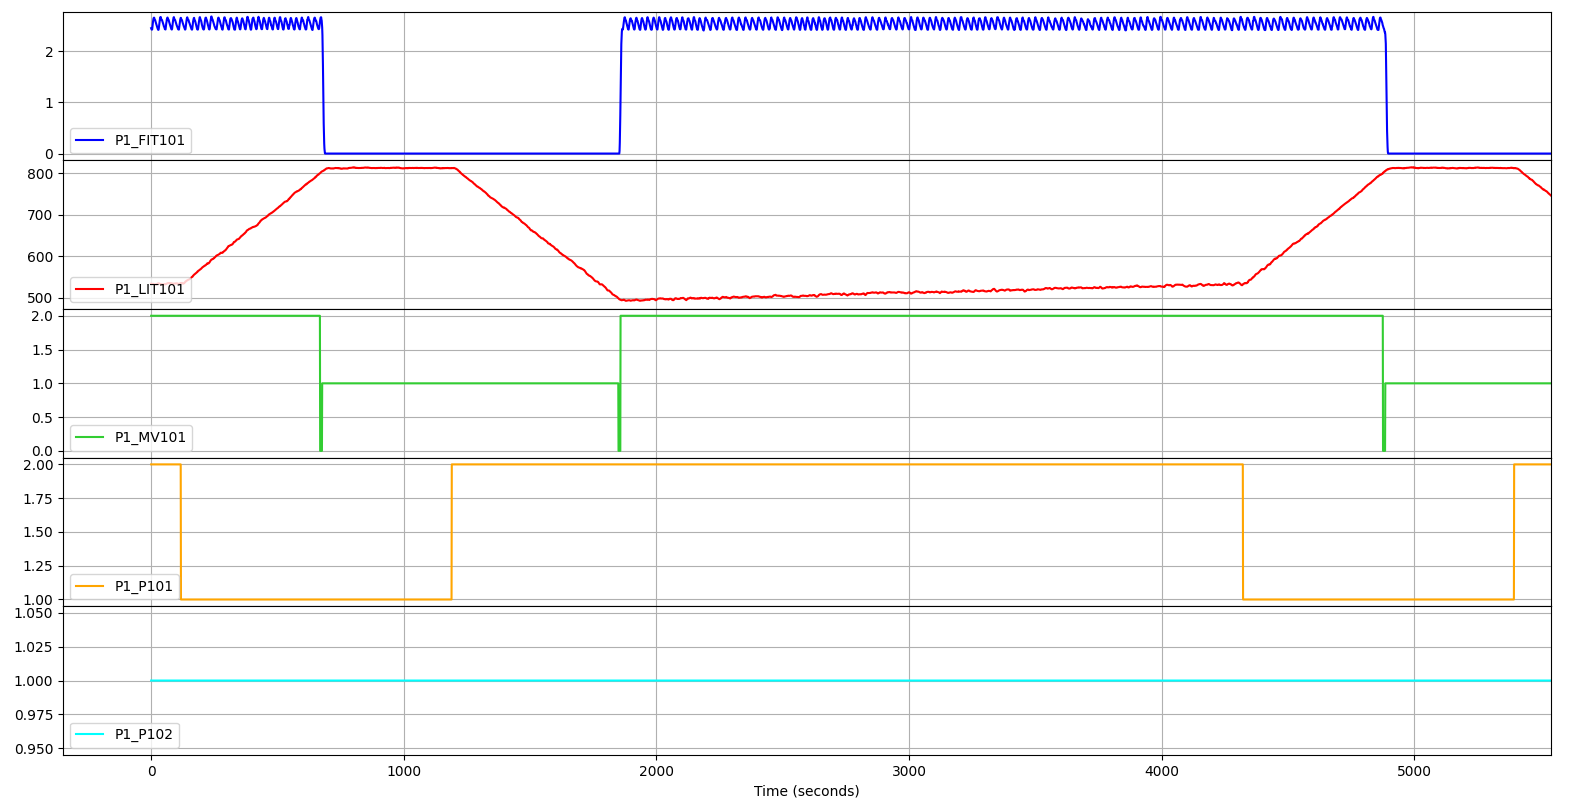
\includegraphics[width=\textwidth]{chap4/graph_analysis_plot_2.png}
		\caption{Zooming on a particular zone of the charts}
		\label{subfig:4_graph_analysis_2}
	\end{subfigure}
	\caption{Example of the new graph analysis}
	\label{fig:4_graph_analysis}
\end{figure}

\bigskip
To demonstrate the behavior and effectiveness of the new graph analysis process, we observe in particular, Figure \ref{subfig:4_graph_analysis_2}: we can already have some validation on the conjectures made in the preliminar analysis from the previous step:

\begin{itemize}
	\item the data presented in the \texttt{P1\_FIT101} chart provides support for associating this register with a \textbf{measurement}. Furthermore, the chart indicates a close correlation between the trend of this register and the periods in which \texttt{P1\_LIT101} exhibits an upward trend and the evolution of \texttt{P1\_MV101}. The values of \texttt{P1\_FIT101}, ranging from approximately 0 to 2.5, are too limited to conclude that this register represents the level sensor of a tank. The overall trend also aligns with this interpretation, suggesting that it is more likely a \textbf{pressure or flow sensor};
	
	\item based on the information provided above, it appears that \texttt{P1\_LIT101} indeed \textbf{represents the level sensor of a tank}, which was initially assumed in the preliminar analysis. The hypothesis is further reinforced by several factors. Firstly, the wide range of values observed in this register supports the notion of it being a level sensor. Additionally, the graphical representation of the level trend provides valuable insights. It shows an initial sharp rise, followed by a period of stabilization referred to as a \textit{plateau}, and subsequently, a similarly steep descent. Finally, there is a new phase of slower level growth compared to the previous one. These patterns lend further support to the interpretation of \texttt{P1\_LIT101} as a sensor specifically measuring the level of a tank;
	
	\item at the start of the ascending trend of \texttt{P1\_LIT101}, the value of \texttt{P1\_MV101} is 2. Conversely, during the \textit{plateau} phase observed when the measurement is approximately 800 and during the descending trend, \texttt{P1\_MV101} has a value of 1. These observations provide further confirmation of the initial hypothesis: the value 1 represents the \textbf{OFF state} of the sensor, while 2 represents the \textbf{ON state}. Moreover, \texttt{P1\_MV101} can be identified as the actuator responsible for causing the rising level in \texttt{P1\_LIT101};
	
	\item during the preliminar analysis, we noticed the short duration of \texttt{P1\_MV101} in state 0, but we were unable to speculate on the underlying reason. However, further analysis of the graph reveals that \texttt{P1\_MV101} transitions and remains in the 0 state, acting as a type of "transient" between states 1 and 2. It can be inferred that this period represents the actual time required for the actuator to change its state.
	
	\item we can observe the behavior of \texttt{P1\_P101} in relation to \texttt{P1\_LIT101} and \texttt{P1\_MV101} to understand its role. At the beginning of the descending trend of \texttt{P1\_LIT101}, after the plateau phase, \texttt{P1\_P101} assumes a value of 2. It then changes back to value 1 at the point of the (presumed) tank's level increase. Although this fact alone may not be entirely clear, when comparing the behaviors of \texttt{P1\_P101}, \texttt{P1\_LIT101}, and \texttt{P1\_MV101}, certain patterns emerge. When \texttt{P1\_P101} and \texttt{P1\_MV101} are both in state 1, the water level remains stable. However, when P1\_P101 changes to state 2, the level of the measurement drops rapidly. Subsequently, when P1\_MV101 also transitions to state 2, the level slowly starts to rise again, with a sudden increase occurring when \texttt{P1\_P101} changes from 2 back to 1. From these observations, it can be inferred that \texttt{P1\_P101} serves as the \textbf{actuator responsible for emptying the presumed tank}. State 1 represents the \textbf{OFF state}, while state 2 represents the \textbf{ON state} of this actuator.
	
	\item it appears that \texttt{P1\_P102} plays no active role in the system as its state remains constant at 1 throughout. Considering this information, it seems unlikely that \texttt{P1\_P102} could serve as a relative setpoint. Therefore, according to the preliminar analysis, it can be inferred that \texttt{P1\_P102} is most likely a \textbf{spare actuator} that is not actively utilized in the system. A \textit{spare actuator} is indeed a secondary actuator that is intended to remains idle unless needed as a backup or replacement when the primary actuator is unavailable or needs to be taken out of service.
\end{itemize}

\bigskip
As the reader has probably already noticed, the majority of the graphs presented in the previous sections and chapters were generated using the new graph analysis script, specifically the \texttt{runChartsSubPlots.py} script. This Python script is located in the \texttt{\$(project-dir)/statistical-graphs} directory and utilizes the \textit{matplotlib} libraries to generate the graph plots, similar to the previous tool.\newline 
The script accepts the following command-line parameters:

\begin{itemize}
	\item \textbf{-f} or \textbf{{-}{-}filename}: specifies the CVS format dataset to read data from. The dataset must be within the directory containing the enriched datasets for the invariant analysis phase. If subsequent parameters are not specified, the script will display all registers in the dataset, excluding any additional attributes;
	
	\item \textbf{-r} or \textbf{{-}{-}registers}: specifies one or more specific registers to be displayed;
	
	\item \textbf{-a} or \textbf{{-}{-}addregisters}: adds one or more registers to the default visualization. This option is useful in case an additional attribute such as slope is to be analyzed;
	
	\item \textbf{-e} or \textbf{{-}{-}excluderegisters}: excludes one or more specific registers from the default visualization. This option is useful to avoid displaying hardcoded setpoints or spare registers.
\end{itemize}
This script, like the previous ones, is designed to provide the maximum flexibility and ease of use for the user, combined with greater power and effectiveness in deriving useful information about the analyzed system.

\paragraph{Statistical Analysis} After careful consideration, we made the decision not to include the statistical analysis aspect of the previous tool in the framework. We found that there was no practical use for it. Instead, we integrated the relevant statistical information into the preliminar analysis conducted after the pre-processing phase. Additionally, we deemed the histogram to have limited utility and considered it outdated in comparison to the new graph analysis approach we implemented. \newline
Although we decided not to include the statistical analysis aspect in the framework, the Python script \texttt{histPlots\_Stats.py} from the original tool remains in the directory. This script is essentially unchanged from the version developed by Ceccato et al. and can be used in the future if the need arises. 

\subsection{Phase 3: Invariant Inference and Analysis}
\label{subsec:4_improve_invariants}
The phase of invariant inference and analysis has undergone a redesign and improvement to offer the user a more comprehensive and easier approach to identify invariants. This has been achieved through the application of new criteria to analyze and reorganize the Daikon analysis results. The outcome of this is a more compact presentation of information that highlights the possible relationships among invariants.\newline
The new design not only enables the identification of undiscovered aspects of the system behavior but also confirms the hypotheses made during the earlier stages of analysis. This step is now semi-automated, unlike before, and allows for the analysis of invariants on individual actuator states and their combinations.

\subsubsection{Revised Daikon Output}
\label{subsub:4_new_daikon_output}
To streamline the process of identifying invariants quickly and efficiently, it is necessary to revise the output generated by standard Daikon analysis. The goal is to create a more compact and readable format for the output.
\newline \newline
The current Daikon results basically consist of three sections, referred as \textit{program point sections} \cite{daikon_program_point}:

\begin{enumerate}
	\item the first section containing generic invariants, i.e., valid regardless of whether a condition is specified for the analysis;
	
	\item the second section containing invariants obtained by specifying a condition for the analysis in the \textit{.spinfo} file, if any;
	
	\item a third section containing the invariants that are obtained from the negation of the condition potentially specified in the \textit{.spinfo} file.
\end{enumerate}

In each section only a single invariant per row is shown, without relating it in any way to the others: this makes it difficult to identify significant invariants and any invariant chain that might provide much more information about the behavior of the system than the single invariant.\newline
A brief example of the structure and format of this output related to \texttt{PLC1} of the iTrust SWaT system is shown in Listing \ref{lst:4_daikon_output_plc1}, where a condition was specified on the measurement \texttt{P1\_LIT101} and on actuator \texttt{P1\_MV101}: % sono 61 righe effettive di invarianti - 48 generiche, 10 condizionali, 1 negata

\begin{lstlisting}[language=bash,numbers=none,caption={Standard Daikon output for \texttt{PLC1} of the iTrust SWaT system},label=lst:4_daikon_output_plc1]
	aprogram.point:::POINT
	P1_P102 == prev_P1_P102
	P1_FIT101 >= 0.0
	P1_MV101 one of { 0.0, 1.0, 2.0 }
	P1_P101 one of { 1.0, 2.0 }
	P1_P102 == 1.0
	max_P1_LIT101 == 816.0
	min_P1_LIT101 == 489.0
	slope_P1_LIT101 one of { -1.0, 0.0, 1.0 }
	[...]
	P1_LIT101 > P1_MV101
	P1_LIT101 > P1_P101
	P1_LIT101 > P1_P102
	P1_LIT101 < max_P1_LIT101
	P1_LIT101 > min_P1_LIT101
	[...]
	P1_MV101 < min_P1_LIT101
	P1_MV101 < trend_P1_LIT101
	P1_P101 >= P1_P102
	P1_P101 < max_P1_LIT101
	[...]
  ===============================================
	aprogram.point:::POINT;condition="P1_MV101 == 2.0 && P1_LIT101 < max_P1_LIT101 - 16 && P1_LIT101 > min_P1_LIT101 + 15"
	P1_MV101 == prev_P1_MV101
	P1_P102 == slope_P1_LIT101
	P1_MV101 == 2.0
	P1_FIT101 > P1_MV101
	P1_FIT101 > P1_P101
	P1_FIT101 > P1_P102
	P1_FIT101 > prev_P1_P101
	P1_MV101 >= P1_P101
	P1_MV101 >= prev_P1_P101
	P1_P101 <= prev_P1_P101
  ===============================================
	aprogram.point:::POINT;condition="not(P1_MV101 == 2.0 && P1_LIT101 < max_P1_LIT101 - 16 && P1_LIT101 > min_P1_LIT101 + 15)"
	P1_P101 >= prev_P1_P101
	Exiting Daikon.
\end{lstlisting}

In the presented framework, the output is simplified to \textbf{two sections}: the \textit{general section} and the section related to the \textit{user-specified condition}. The section related to the negated condition is eliminated as it is not relevant in this context and could lead to potential misinterpretation. Moreover, the relationships between invariants will be emphasized by utilizing \textbf{transitive closures}: transitive closure of a relation $R$ is another relation, typically denoted $R^{+}$ that adds to $R$ all those elements that, while not necessarily related directly to each other, can be reached by a \textit{chain} of elements related to each other. In other words, the transitive closure of $R$ is the smallest (in set theory sense) transitive relation $R$ such that $R$ $\subset$ $R^{+}$ \cite{transitive_closures}. 

\bigskip
To implement the transitive closure of the invariants generated by Daikon, we initially categorized the invariants in each section by type based on their mathematical relation ($==$, $>$, $<$, $>=$, $<=$, $!=$), excluding any invariant related to additional attributes except for the slope. For each type of invariant, we constructed a \textbf{graph} using the NetworkX library, where registers were represented as nodes, and arcs were created to connect registers that shared a common endpoint in the invariant, applying the transitive property. To reconstruct the individual invariant chains, we employed a straightforward approach known as \textit{Depth-first Search} (DFS) on each of the graphs. This method allowed us to traverse the graphs and obtain the desired outcome, identifying the invariant chains. Figure \ref{fig:4_transitive_closure_graphs} shows some examples of these graphs:

\begin{figure}[H]
	\centering
	\begin{subfigure}{0.48\textwidth}
		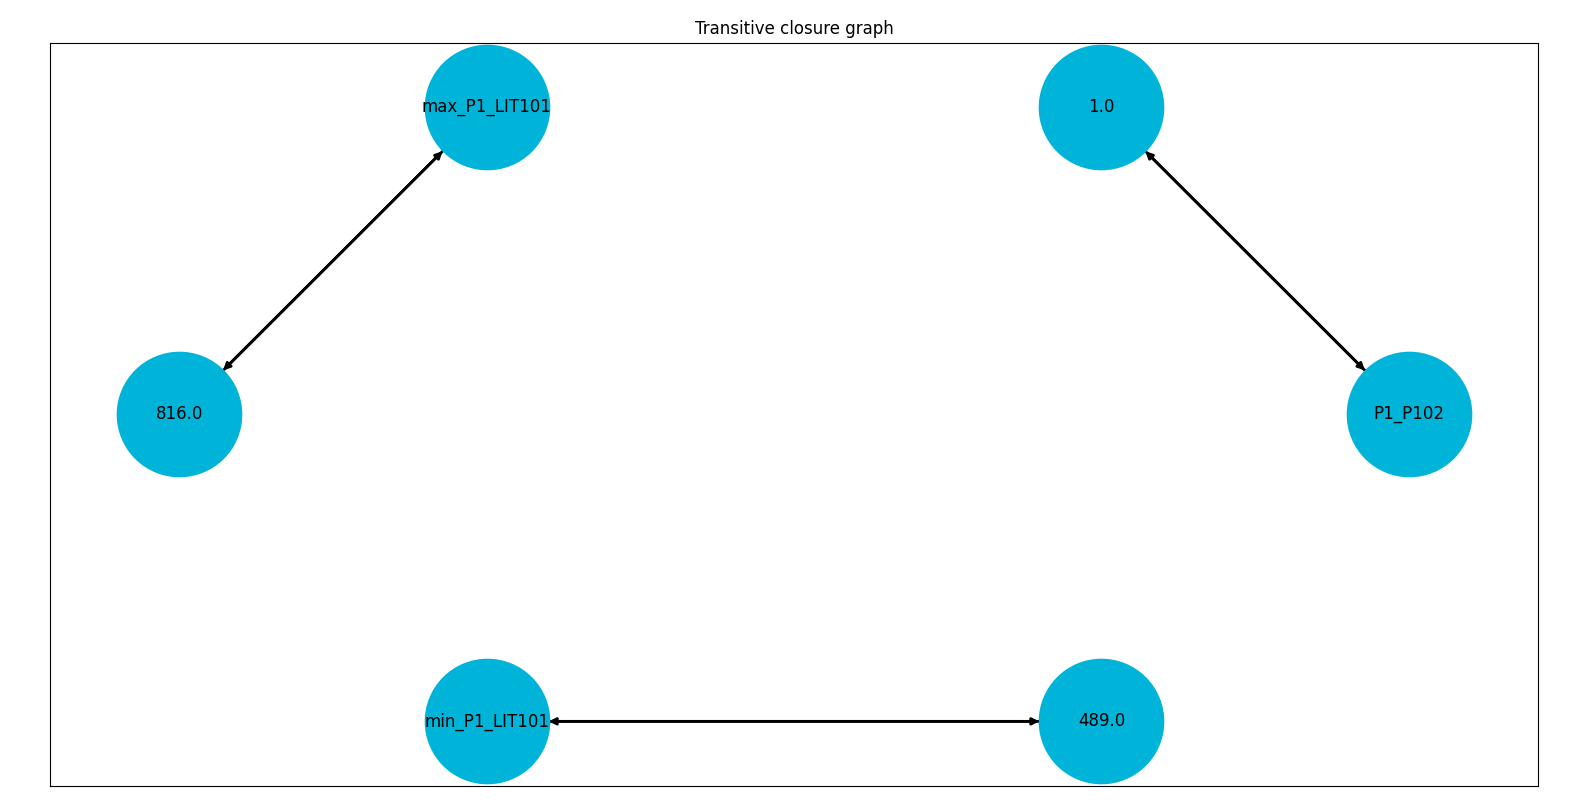
\includegraphics[width=\textwidth]{chap4/transitive_closure_eq.png}
		\caption{Transitive closure graph for "=="}
		\label{subfig:4_graph_eq}
	\end{subfigure}
	\hfill
	\begin{subfigure}{0.48\textwidth}
		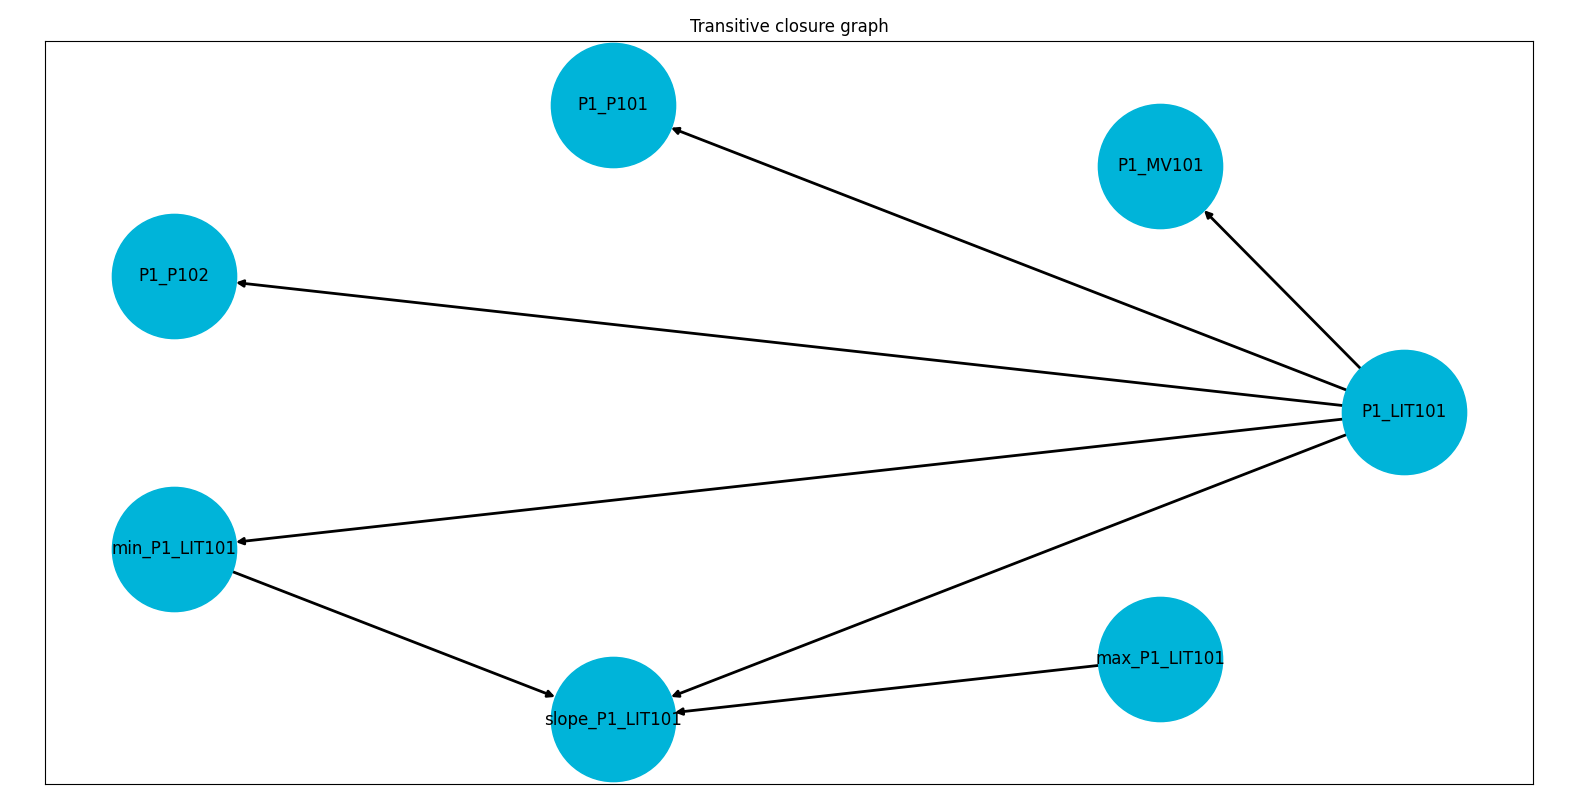
\includegraphics[width=\textwidth]{chap4/transitive_closure_gt.png}
		\caption{Transitive closure graph for ">"}
		\label{subfig:4_graph_gt}
	\end{subfigure}
	\begin{subfigure}{0.48\textwidth}
		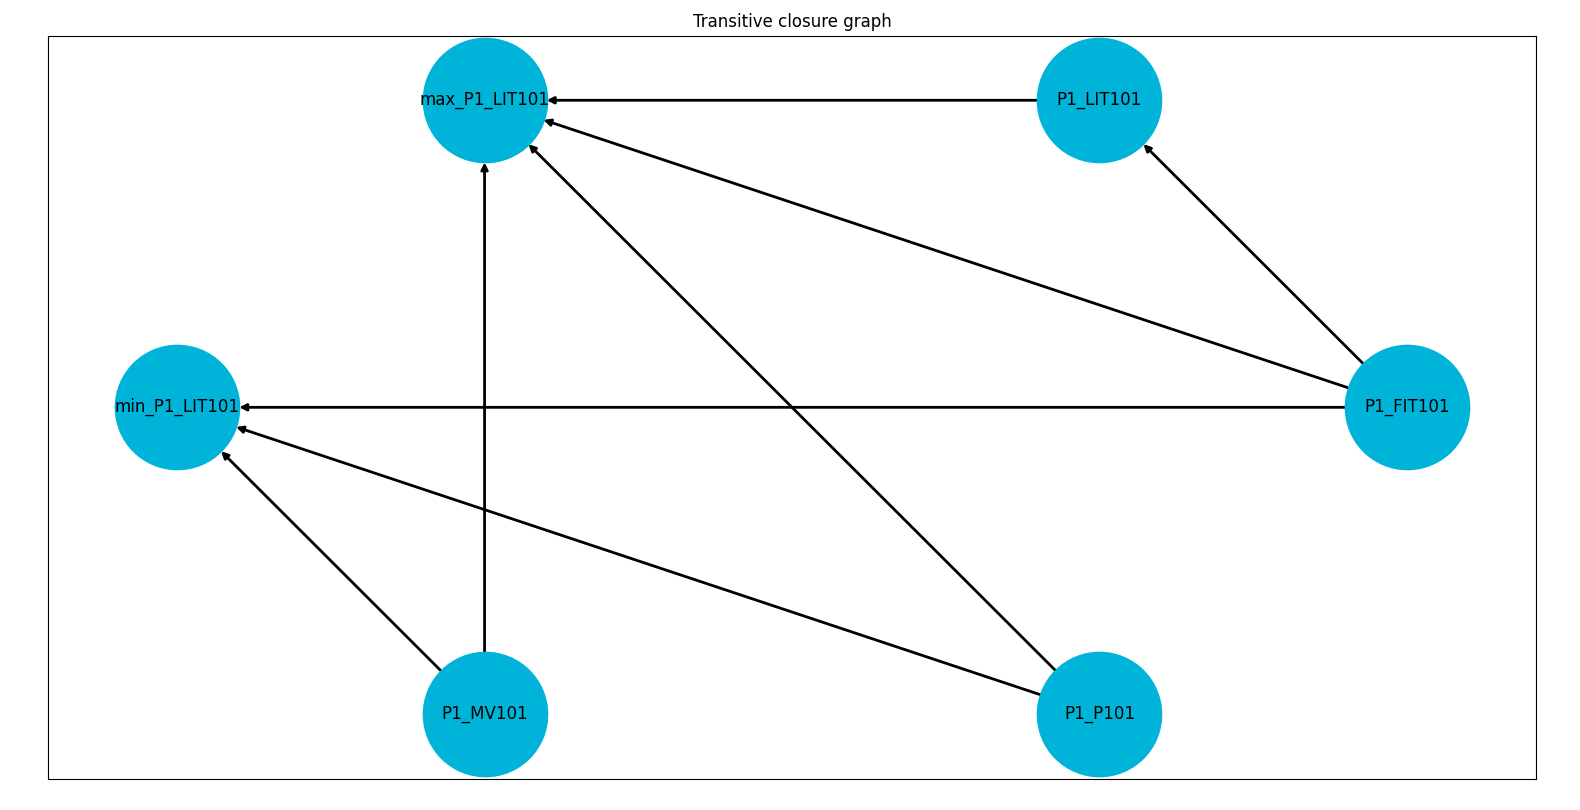
\includegraphics[width=\textwidth]{chap4/transitive_closure_lt.png}
		\caption{Transitive closure graph for "<"}
		\label{subfig:4_graph_lt}
	\end{subfigure}
	\hfill
	\begin{subfigure}{0.48\textwidth}
		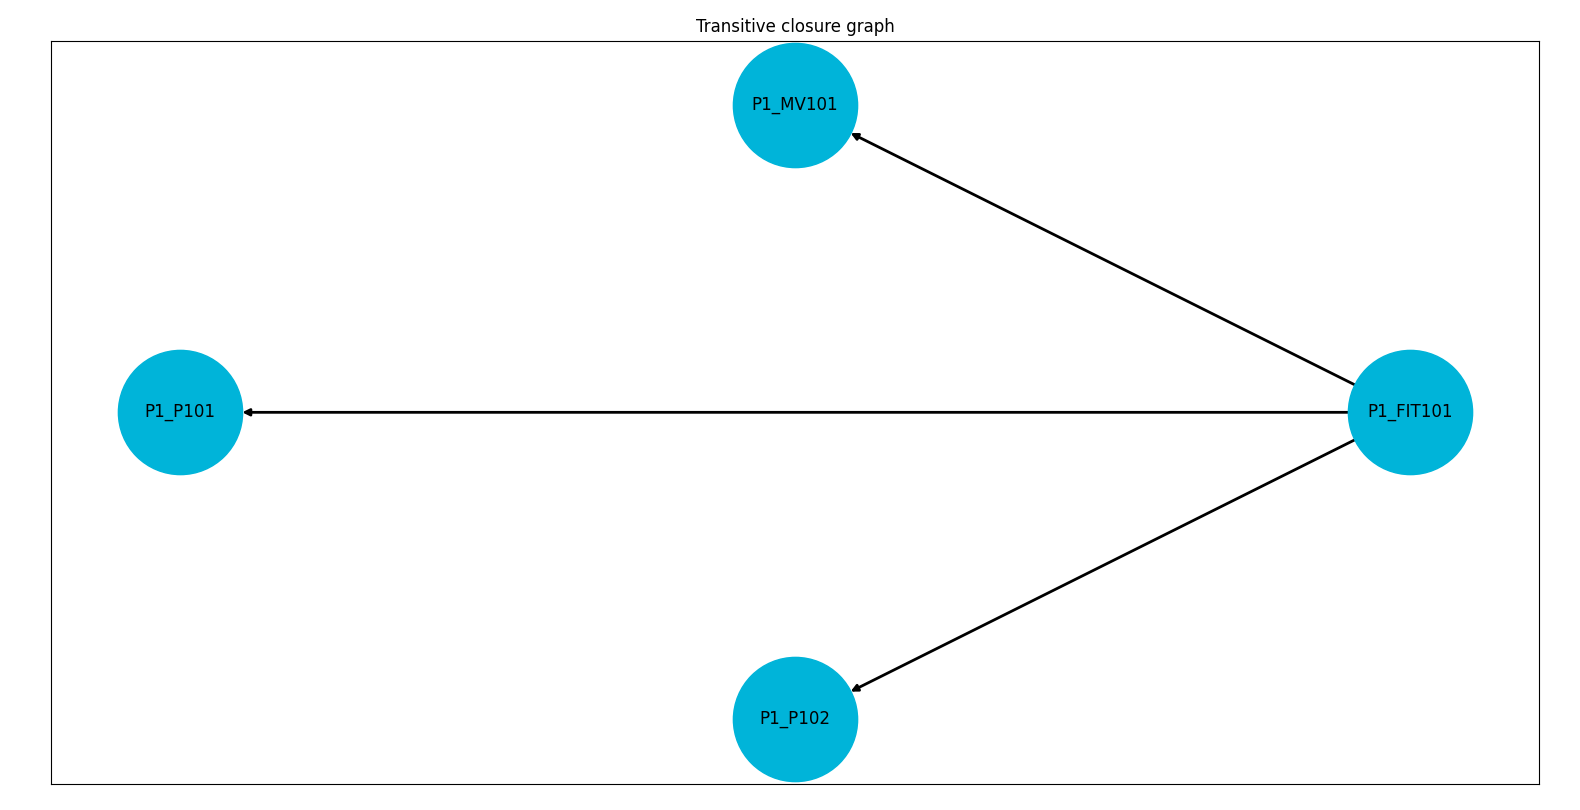
\includegraphics[width=\textwidth]{chap4/transitive_closure_gt_cond.png}
		\caption{Transitive closure graph for ">" cond.}
		\label{subfig:4_graph_gt_cond}
	\end{subfigure}
	\caption{Example of transitive closure graphs for invariants in PLC1 of iTrust SWaT system}
	\label{fig:4_transitive_closure_graphs}
\end{figure}
At the end of this process, still applied to \texttt{PLC1} of the iTrust SWaT system and with the same analysis condition, we get the following complete output:

\begin{lstlisting}[language=bash,numbers=left,caption={Revised Daikon output with transitive closures for \texttt{PLC1} of the iTrust SWaT system},label=lst:4_daikon_new_output_plc1]
	===========================
	Generic
	===========================
	P1_MV101 one of { 0.0, 1.0, 2.0 }
	P1_P101 one of { 1.0, 2.0 }
	slope_P1_LIT101 one of { -1.0, 0.0, 1.0 }
	P1_FIT101 != P1_P101, P1_P102
	P1_P102 == 1.0
	max_P1_LIT101 == 816.0
	min_P1_LIT101 == 489.0
	P1_LIT101 > P1_MV101
	P1_LIT101 > P1_P101
	P1_LIT101 > P1_P102
	P1_LIT101 > min_P1_LIT101 > slope_P1_LIT101
	P1_FIT101 >= 0.0
	P1_P101 >= P1_P102 >= slope_P1_LIT101
	
	===========================
	P1_MV101 == 2.0 && P1_LIT101 < max_P1_LIT101 - 16 && P1_LIT101 > min_P1_LIT101 + 15
	===========================
	slope_P1_LIT101 == P1_P102
	P1_MV101 == 2.0
	P1_FIT101 > P1_MV101
	P1_FIT101 > P1_P101
	P1_FIT101 > P1_P102
	P1_MV101 >= P1_P101
\end{lstlisting}
Transitive closures can be appreciated in lines 7, 14 and 16 of Listing \ref{lst:4_daikon_new_output_plc1}.\newline
In general, the output has been reduced in the number of effective rows (19 versus the 61 in the output of Listing \ref{lst:4_daikon_output_plc1}, making it certainly better to read and identify significant invariants) and the invariant chains make it more immediate to grasp the relationships between registers.

\subsubsection{Types of Analysis}
\label{subsub:4_types_analysis}

In contrast to Ceccato et al.'s solution, which involves manual individual analyses, our proposal is to introduce \textbf{two types of semi-automated analysis}.\newline 
The first type focuses on analyzing \textbf{all states for each individual actuator}. This automated analysis aims to provide comprehensive insights into the behavior of each actuator in relation to a specific measurement selected by the user.\newline
The second type of analysis considers the current system configuration and examines the \textbf{actual states of the actuators}. This analysis takes into account the interplay and combined effects of multiple actuators on the selected measurement. By incorporating the real-time states of the actuators, this semi-automated analysis offers a more accurate assessment of the system behavior.

\bigskip
These two types of analysis will be handled by the Python script\\ \texttt{daikonAnalysis.py}, contained in the default directory \texttt{\$(project\_dir)/daikon}.\newline
The script accepts the following command-line arguments:

\begin{itemize}
	\item \textbf{-f} or \textbf{{-}{-}filename}: specifies the enriched dataset, in CSV format, from which to read the data. The dataset must be located within the directory containing the enriched datasets specified in the \textit{config.ini} file (by default \texttt{\$(project\_dir)/daikon/Daikon\_Invariants});
	
	\item \textbf{-s} or \textbf{{-}{-}simpleanalysis}: performs the analysis on the states of individual actuators;
	
	\item \textbf{-c} or \textbf{{-}{-}customanalysis}: performs the analysis on combinations of actual states of the actuators;
	
	\item \textbf{-u} or \textbf{{-}{-}uppermargin}: defines a percentage margin on the maximum value of the measurement;
	
	\item \textbf{-l} or \textbf{{-}{-}lowermargin}: defines a percentage margin on the minimum value of the measurement;
\end{itemize}
The selection of one or both types of analysis is possible. Additionally, the last two parameters can be used to set a condition on the value of the measurement. This condition is designed to bypass the transient periods that occur during actuator state changes and the actual trend changes at the maximum and minimum values of the measurement.\newline
This approach proves particularly beneficial for the first type of analysis, as it enables more accurate data on the trends of the measurement. By excluding the transient periods, the analysis can focus on the stable and meaningful trends, providing improved insights into the behavior of the system.

\paragraph{Analysis on single actuator states}
\label{par:4_single_actuator_states_analysis}
Analysis on the states of individual actuators is the simplest: after the user is prompted to input the measurement, chosen from a list of likely available measurements, the script recognizes the likely actuators and the relative states of each, using the same mixed Daikon/Pandas technique adopted in the preliminar analysis during the pre-processing phase.\newline
For each actuator and each state it assumes, a single Daikon analysis is performed, eventually placing the condition on the maximum and minimum level of the measurement.\newline 
The result of these analyses are saved in the form of text files in a directory having the name corresponding to the analyzed actuator and contained in the default parent directory \texttt{\$(project\_dir)/daikon/Daikon\_Invariants/results}: each file generated by the analysis is identified by the name of the actuator, the state and the condition, if any, on the measurement (see Figure \ref{fig:4_daikon_simpleanalysis_dirfiles}).

\begin{figure}[H]
	\centering
	\begin{subfigure}{0.48\textwidth}
		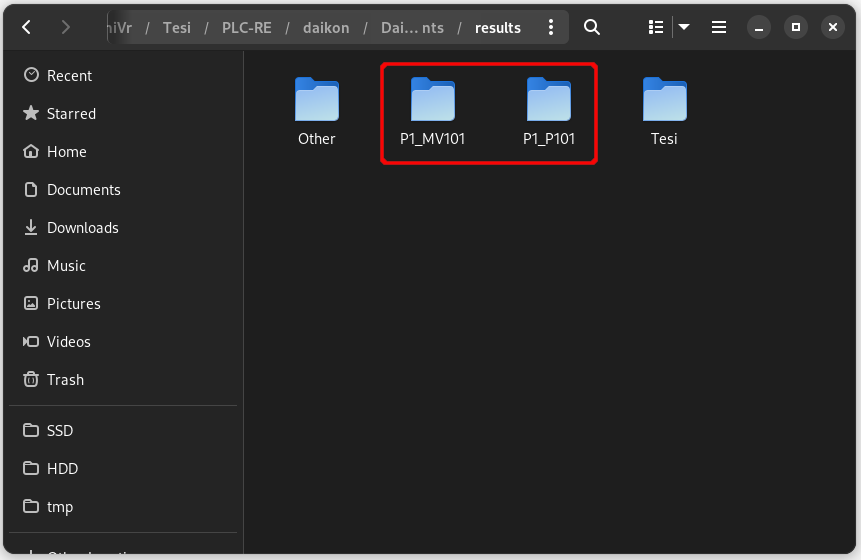
\includegraphics[width=\textwidth]{chap4/daikon_resultfiles_dirs.png}
		\caption{}
		\label{subfig:4_daikon_results_dir}
	\end{subfigure}
	\hfill
	\begin{subfigure}{0.48\textwidth}
		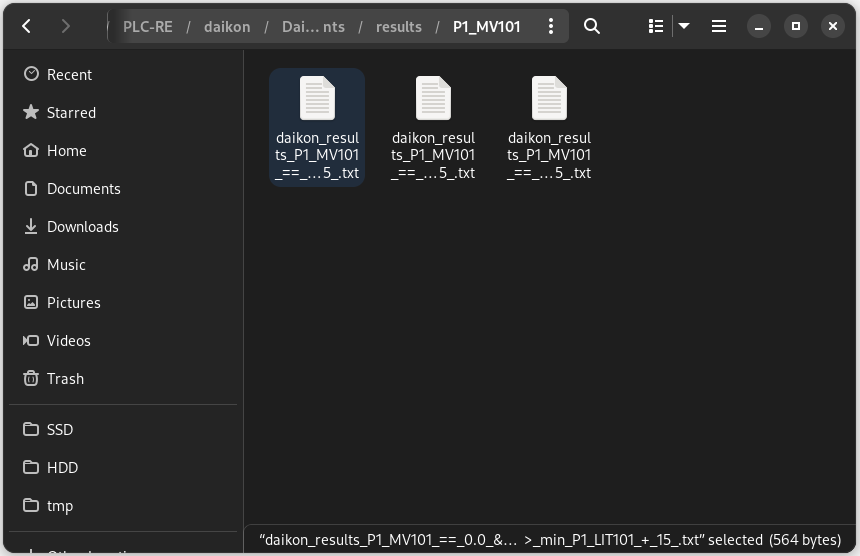
\includegraphics[width=\textwidth]{chap4/actuator_analysis_files.png}
		\caption{}
		\label{subfig:4_daikon_results_file}
	\end{subfigure}
	\caption{Directory (a) and outcome files (b) for the single actuator states analysis}
	\label{fig:4_daikon_simpleanalysis_dirfiles}
\end{figure}

Listing \ref{lst:4_daikon_new_output_plc1} provides an illustrative example of the analysis results. In this case, we focus on the actuator \texttt{P1\_MV101} in state 2. By examining the generic invariants, we can deduce that \texttt{P1\_P101} is a probable actuator with binary values, as indicated in line 5. However, upon closer inspection in line 8, we discover that \texttt{P1\_P102} consistently maintains a value of 1 throughout, thus confirming its role as a spare actuator rather than a setpoint. Furthermore, lines 9 and 10 present the maximum and minimum values achieved by \texttt{P1\_LIT101}, the register presumed to be connected to the tank.\newline
The condition-generated invariants provide the most interesting insights. In particular, at line 21, we observe that when \texttt{P1\_MV101} is set to 2, the slope of \texttt{P1\_LIT101} is 1, indicating an increasing trend. This confirms our previous assumption that \texttt{P1\_MV101} represents the actuator's ON state and is responsible for filling the tank (\texttt{P1\_LIT101}).\newline
Furthermore, at line 23, we discover that \texttt{P1\_FIT101} is greater than \texttt{P1\_MV101}. This implies that when the actuator assumes the value 2, the sensor \texttt{P1\_FIT101} registers a measurement. In contrast, when \texttt{P1\_MV101} is 1, \texttt{P1\_FIT101} remains at 0, signifying no recorded readings. This finding reinforces our initial hypothesis that \texttt{P1\_FIT101} may serve as a pressure or flow sensor.

\paragraph{Analysis of the Current System Configuration}
\label{par:4_current_system_config_analysis}
The analysis of the current system configuration based on the actual states of the actuators is more complex, but at the same time offers more interesting outcomes as it provides better evidence of actuator behavior in relation to the selected measurement.

\begin{figure}[H]
	\centering
	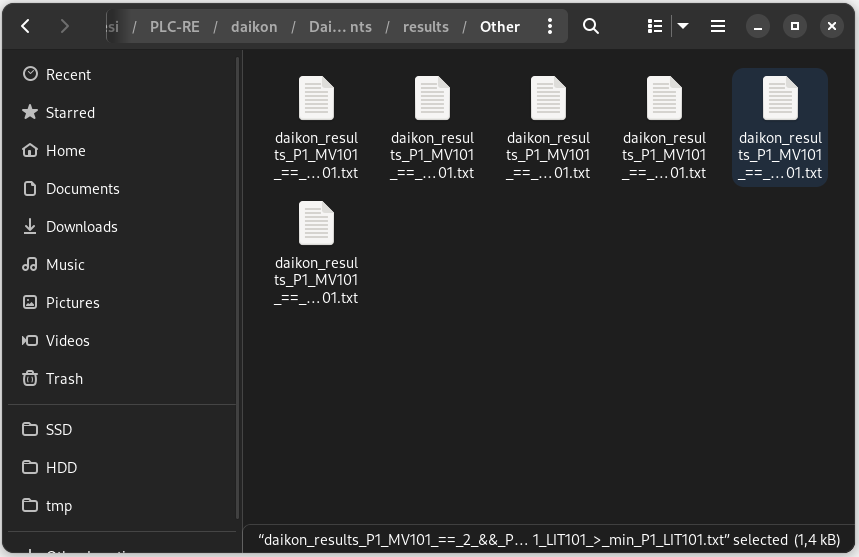
\includegraphics[scale=0.35]{chap4/daikon_systemstate_results.png}
	\caption{Daikon outcome files for system configuration analysis. Each file represents a single system state}
	\label{fig:4_daikon_systemstates_files}
\end{figure}

For this analysis, the script automatically identifies the configurations of the actuators that represent different system states (e.g., \texttt{P1\_MV101 == 2, P1\_P101 == 1}). Daikon analysis is then performed for each of these configurations. The user is prompted to select the measurement attribute and, if desired, specific actuators for studying their configurations. If no actuators are selected, all previously detected actuators will be considered.\newline
The analysis results are saved in text format within a designated directory, located alongside the previous analysis outputs. The filenames of these result files follow a specific naming convention based on the analysis rule applied (see Figure \ref{fig:4_daikon_systemstates_files}).\newline \newline
An example of the obtained outcomes can be seen in Listing \ref{lst:4_current_system_config_analysis}:

\begin{lstlisting}[language=bash,numbers=left,caption={Daikon outcomes for the system configuration \texttt{P1\_MV101 == 2, P1\_P101 == 1} on \texttt{P1\_LIT101}},label=lst:4_current_system_config_analysis]
	===========================
	Generic
	===========================
	P1_MV101 <= P1_P101  ==>  P1_FIT101 >= 0.0
	P1_MV101 <= P1_P101  ==>  P1_MV101 one of { 0.0, 1.0, 2.0 }
	P1_MV101 <= P1_P101  ==>  P1_P101 one of { 1.0, 2.0 }
	P1_MV101 <= P1_P101  ==>  slope_P1_LIT101 one of { -1.0, 0.0, 1.0 }
	P1_MV101 > P1_P101  ==>  P1_FIT101 > P1_MV101
	P1_MV101 > P1_P101  ==>  P1_FIT101 > P1_P101
	P1_MV101 > P1_P101  ==>  P1_FIT101 > P1_P102
	P1_MV101 > P1_P101  ==>  P1_FIT101 > slope_P1_LIT101
	P1_MV101 > P1_P101  ==>  P1_MV101 == 2.0
	P1_MV101 > P1_P101  ==>  P1_MV101 > P1_P102
	P1_MV101 > P1_P101  ==>  P1_MV101 > slope_P1_LIT101
	P1_MV101 > P1_P101  ==>  P1_P101 == 1.0
	P1_MV101 > P1_P101  ==>  P1_P101 == P1_P102
	P1_MV101 > P1_P101  ==>  P1_P101 == slope_P1_LIT101
	P1_MV101 > P1_P101  ==>  slope_P1_LIT101 == 1.0
	[...]
	
	===========================
	P1_MV101 == 2 && P1_P101 == 1 && P1_LIT101 < max_P1_LIT101 && P1_LIT101 > min_P1_LIT101
	===========================
	slope_P1_LIT101 == P1_P102 == P1_P101 == 1.0
	P1_MV101 == 2.0
	P1_FIT101 > P1_MV101
	P1_FIT101 > P1_P101
\end{lstlisting}
In contrast to Listing \ref{lst:4_daikon_new_output_plc1}, the current analysis reveals the presence of implications in the general invariants section, which were previously absent (remaining generic invariants omitted for brevity). These implications offer valuable insights, as demonstrated in this case. For instance, the invariant stated in line 18 informs us that if the value of \texttt{P1\_MV101} in greater than \texttt{P1\_P101}, then the slope's value is 1, indicating an increasing tank level. This finding further corroborates our initial understanding that the state \texttt{P1\_MV101 == 2} represents the ON state for the actuator responsible for filling the tank, namely \texttt{P1\_LIT101}. Upon comparing the results of the other analyses, we will uncover that \texttt{P1\_P101} serves the purpose of emptying the tank, with its ON and OFF states denoted as 2 and 1, respectively.\newline 
Furthermore, the invariant presented in line 8 reveals that when \texttt{P1\_MV101} is in state 2 and \texttt{P1\_P101} is in state 1, the value of \texttt{P1\_FIT101} ins greater than 2. Consequently, it can be inferred that the associated sensor is measuring something in relation to the tank represented by \texttt{P1\_LIT101}.\newline
The aforementioned observations are further supported by the invariants associated with the analysis condition. As indicated in line 24, the slope is indeed equal to 1, confirming an upward trend. Additionally, at line 26, it is evident that \texttt{P1\_FIT101} assumes values greater than 2 when \texttt{P1\_MV101} is equal to 2.

\paragraph{Refining the Analysis}
\label{par:4_refining_analysis}
In certain situations, the outcomes provided by the semi-automated analyses may not meet the user's expectations. For instance, the clarity of the slope value may be insufficient, or the user may wish to delve deeper into a specific aspect of the system to uncover additional invariants that were not previously identified. In such cases, the user has the option to conduct a more targeted and specific invariant analysis using the Python script \texttt{runDaikon.py}, which enables precise investigations of the system.\newline
The script, located in the default directory \texttt{\$(project\_dir)/daikon}, can be executed with three command-line parameters:

\begin{itemize}
	\item \textbf{-f} or \textbf{{-}{-}filename}: specifies the CSV format \textit{enriched} dataset to read data from. Even in this case, the dataset must be located within the directory containing the enriched datasets;
	\item \textbf{-c} or \textbf{{-}{-}condition}: specifies the condition for the analysis, which will be automatically overwritten in the \textit{.spinfo} file. It is possible to specify more than one condition, but it is strongly recommended to use the logical operator \texttt{\&\&} to avoid undesired behaviors in Daikon outcomes;
	\item \textbf{-r} or \textbf{{-}{-}register}: specifies the directory where to save the text file with the outcomes.
\end{itemize}
During the execution of this analysis, a single output file is generated, containing the discovered invariants. The user can specify the directory where this file should be saved using the \texttt{-r} command-line option. By default, the file is stored in the directory \texttt{\$(project\_dir)/daikon/Daikon\_Invariants/results}. The output file serves as a record of the identified invariants and can be examined at a later time. 

\bigskip
In conclusion, the integration of these two analysis types, along with the ability to conduct more refined analysis in the future and the enhanced output format of Daikon, significantly enhances the completeness, clarity, and effectiveness of this stage compared to the previous framework.

\subsection{Phase 4: Businness Process Analysis}
\label{subsec:4_improve_bpa}
We have made significant revisions to the Business Process Analysis we are presenting. Instead of relying on the previous Java solution and proprietary process mining software Disco, we have adopted a \textbf{new integrated solution} created in Python from scratch. The new solution utilizes the Graphviz libraries to generate the corresponding activity diagram.\newline \newline
In this updated Business Process, greater emphasis is placed on process mining related to the physical system. Our goal is to extract as much information as possible from the dataset, enabling us to promptly visualize the system's behavior and its various states. This approach allows us to validate the conjectures and hypotheses formulated in the previous phases, and potentially uncover hidden patterns that were previously undisclosed.\newline
On the other hand, the aspect related to network communications was reconsidered to enable operation with multiple protocols, expanding beyond the limitations of Modbus. Unfortunately, despite our intentions, we were unable to implement this modification due to reasons that will be elaborated on later.\newline \newline
Now, let's examine the key aspects of this new phase in greater detail.

\subsubsection{Process Mining of the Physical Process}
\label{subsub:4_proc_minining_phy}

The mining of the physical process is performed by the Python script called \texttt{processMining.py}, located in the default directory \texttt{\$(project\_dir)/process-mining}.\newline
This script accepts the following parameters from the command line:

\begin{itemize}
	\item \textbf{-f} or \textbf{{-}{-}filename:} specifies the CSV format \textit{timestamped} dataset to be mined from. The dataset is obtained from the pre-processing stage and is located in the default directory \texttt{\$(project\_dir)/process-mining/data};
	
	\item \textbf{-a} or \textbf{{-}{-}actuators:} specifies one ore more actuators whose combinations of states are to be analyzed. If this parameter is not provided, all actuators in the subsystem will be considered;
	
	\item \textbf{-s} or \textbf{{-}{-}sensors:} specifies one or more measurements for which the trend will be calculated based on actuator state changes. If this parameter is omitted, all available measurements will be considered;
	
	\item \textbf{-t} or \textbf{{-}{-}tolerance:} specifies the tolerance to be taken into account during the trend calculation; 
	
	\item \textbf{-g} or \textbf{{-}{-}graph:} shows the resulting activity diagram.
\end{itemize}

The script processes the dataset in a sequential manner, analyzing each actuator state change. It calculates the duration in seconds of the system state, as well as the trend and slope of the specified measurement(s). Additionally, the script stores the next system state and the measurement values corresponding to the state change points, allowing for the identification of relative setpoints. These results are gradually collected and stored in a dictionary, where the keys represent the system states based on the actuator configurations, and the values represent the measured values mentioned above. The dictionary is then saved as a JSON file, which can be accessed by the user in the \texttt{\$(project\_dir)/process-mining/data} directory. The name of the file can be specified in the configuration file \textit{config.ini}.\newline \newline
An example of the JSON file obtained in this step is shown in Listing \ref{lst:4_proc_mining_json}: the JSON file showcases the structure of the data obtained during the process.

\begin{lstlisting}[language=java,numbers=none,caption={Example of the data contained in the produced JSON file} ,label=lst:4_proc_mining_json]
	{
		"P1_MV101 == 2, P1_P101 == 2": {
			"start_value_P1_LIT101": [
			534.9366,
			495.4483,
			497.9998,
			495.9586,
			495.8016
			],
			"end_value_P1_LIT101": [
			536.0356,
			532.7384,
			541.7273,
			534.4656,
			540.8245
			],
			"slope_P1_LIT101": [
			0,
			0.015,
			0.018,
			0.016,
			0.018
			],
			"trend_P1_LIT101": [
			"STBL",
			"ASC",
			"ASC",
			"ASC",
			"ASC"
			],
			"time": [
			119,
			2464,
			2477,
			2452,
			2440
			],
			"next_state": [
			"P1_MV101 == 2, P1_P101 == 1",
			"P1_MV101 == 2, P1_P101 == 1",
			"P1_MV101 == 2, P1_P101 == 1",
			"P1_MV101 == 2, P1_P101 == 1",
			"P1_MV101 == 2, P1_P101 == 1"
			]
		},
		"P1_MV101 == 2, P1_P101 == 1": {
			...
		}
		"P1_MV101 == 0, P1_P101 == 1": {
			...
		}
		
		...
	}
\end{lstlisting}

The collected data is now utilized to generate the \textbf{system activity diagram}. This diagram represents an \textit{oriented} graph where the nodes correspond to the system states determined by the actuator configurations. In addition to the state information, the nodes also display the trend (ascending, descending, or stable) and the slope of the reference measurement.\newline
The edges in the diagram depict the values of the measurements at the time of the state change. These measurement values represent the setpoints for each measurement. Setpoints are calculated on the average of the values measured for that specific state. Additionally, the diagram incorporates on the edges the average duration of each system state.\newline
Each data point on the arcs is accompanied by a \textit{standard deviation value}. This value provides information about the occurrence of a specific state within the system's cycle, indicating whether it appears multiple times with varying values and time durations. A low standard deviation suggests that the state is likely to occur only once within each cycle. Conversely, a high standard deviation indicates that the state may occur multiple times within the cycle.

\bigskip
An example of the activity diagram generated by the \texttt{processMining.py} script is presented in Figure \ref{fig:4_process_mining_graph}. This diagram illustrates the system's behavior by depicting transitions between different states. Nodes in the diagram represent specific system states, while arrows or edges indicate the flow between these states.

\begin{figure}[ht]
	\centering
	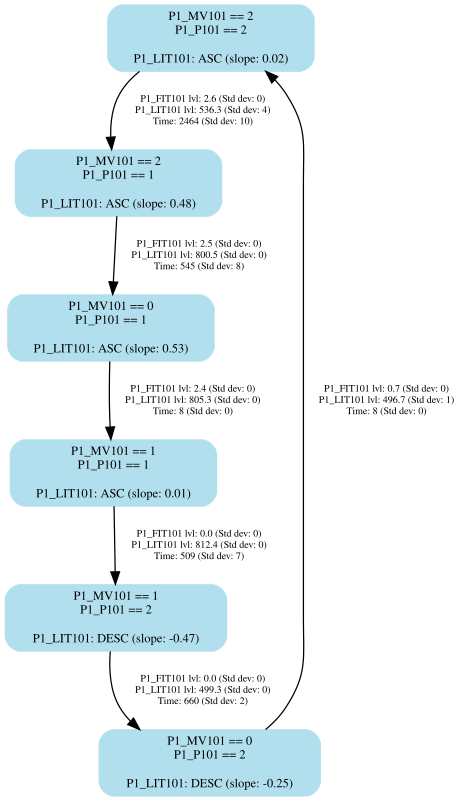
\includegraphics[scale=0.60]{chap4/state_graph_P1_LIT101.png}
	\caption{Activity diagram for PLC1 of the iTrust SWaT system}
	\label{fig:4_process_mining_graph}
\end{figure}

\noindent The diagram reveals important aspects of the system, such as its cyclicality and the emphasis on the temporal sequence of actuator states. These insights might not have been clearly evident in earlier stages of the analysis. The diagram provides a visual representation that allows us to appreciate the recurring patterns and understand how the system evolves over time. By observing the transitions and relationships between different states, we gain a better understanding of the dynamics and behavior of the system.

\bigskip
It is important to acknowledge that despite considering the tolerance set for trend and slope calculation, the accuracy of the related data may vary. For instance, there could be instances where multiple trends exist within the same node, or a trend may be stable instead of increasing or decreasing. These discrepancies arise due to data perturbations, which were discussed in Section \ref{par:4_slope_calculation}. Additionally, smoothing techniques were not employed in this analysis. Therefore, it becomes the responsibility of the user to correctly interpret the outcomes of this step, taking into account the information presented in the process mining diagram and the findings from previous analyses. By considering these factors together, the user can make informed interpretations and draw accurate conclusions from the results.

\subsubsection{Network Communications}
\label{subsub:4_proc_mining_net}
The incorporation of network communications into Business Process Analysis has been reconsidered to shift away from a \textit{single-protocol} solution based on Modbus. Instead, the focus is on adopting a solution that can handle \textbf{multiple protocols}, even at the same time.\newline
The main concept was to develop a new Python script that would extract and process data from PCAP files obtained through network traffic sniffing. The intention was to export this data to a CSV file, which would then be used as input for the process mining script, \texttt{processMining.py}, and integrated with the physical system data to derive commands to the actuators.

%\bigskip
%However, due to the specific case study discussed in Chapter \ref{casestudy} (and especially in Section \ref{subsec:5_2015_datasets}), \textbf{it was not feasible to implement this solution at the time}. The network data available for analysis either lacked references to the reads or writes performed by the actuators or, if such references existed, they were not associated with a suitable physical process dataset for the intended purposes. As a result, the integration of network data with the physical system data could not be realized in the given context.

\bigskip
%Nevertheless, a thorough study was conducted on the available PCAP files to explore potential methodologies that could be implemented as future work. 
The analysis of the network data revealed that different protocols exhibit distinct behaviors when commanding changes in actuator states. Consequently, the previous approach proposed by Ceccato et al. becomes \textbf{impractical} when attempting to detect system state changes through network commands sent to the actuators.\newline
However, considering that system state changes have already been identified through the process mining of the physical process, and with the corresponding event timestamps available, we propose an alternative approach to Ceccato et al.'s method. Instead of seeking the correspondence between network events and physical process events at the same instant, we suggest reversing the perspective. By focusing on the correspondence between a given event occurring in the physical process at a specific moment and the corresponding event in the network data at the same moment, it should be possible to achieve a similar, if not superior, outcome compared to the previous solution.\newline
This \textit{inverse approach} aims to leverage the existing knowledge of system state changes obtained through the mining of the physical process. By aligning these physical events with their corresponding events in the network data, a more effective analysis can be conducted.

%\bigskip
%Although the integration of network data within Business Process Analysis was not feasible, the progress made thus far has resulted in the development of a \textbf{novel form of network analysis}. This approach, unlike the work conducted by Ceccato et al., offers a broader perspective on network communications and delves into previously unexplored aspects of the system. These additional dimensions provide a deeper understanding of the system's behavior and characteristics.\newline
%In the upcoming section, we will delve further into this new network analysis methodology, discussing its unique features and the insights it can offer. By expanding the scope of our analysis, we aim to uncover valuable information that was not extensively explored in previous studies conducted by Ceccato et al.

\vfill
\nolinenumbers